
%% bare_jrnl_compsoc.tex
%% V1.4a
%% 2014/09/17
%% by Michael Shell
%% See:
%% http://www.michaelshell.org/
%% for current contact information.
%%
%% This is a skeleton file demonstrating the use of IEEEtran.cls
%% (requires IEEEtran.cls version 1.8a or later) with an IEEE
%% Computer Society journal paper.
%%
%% Support sites:
%% http://www.michaelshell.org/tex/ieeetran/
%% http://www.ctan.org/tex-archive/macros/latex/contrib/IEEEtran/
%% and
%% http://www.ieee.org/

%%*************************************************************************
%% Legal Notice:
%% This code is offered as-is without any warranty either expressed or
%% implied; without even the implied warranty of MERCHANTABILITY or
%% FITNESS FOR A PARTICULAR PURPOSE! 
%% User assumes all risk.
%% In no event shall IEEE or any contributor to this code be liable for
%% any damages or losses, including, but not limited to, incidental,
%% consequential, or any other damages, resulting from the use or misuse
%% of any information contained here.
%%
%% All comments are the opinions of their respective authors and are not
%% necessarily endorsed by the IEEE.
%%
%% This work is distributed under the LaTeX Project Public License (LPPL)
%% ( http://www.latex-project.org/ ) version 1.3, and may be freely used,
%% distributed and modified. A copy of the LPPL, version 1.3, is included
%% in the base LaTeX documentation of all distributions of LaTeX released
%% 2003/12/01 or later.
%% Retain all contribution notices and credits.
%% ** Modified files should be clearly indicated as such, including  **
%% ** renaming them and changing author support contact information. **
%%
%% File list of work: IEEEtran.cls, IEEEtran_HOWTO.pdf, bare_adv.tex,
%%                    bare_conf.tex, bare_jrnl.tex, bare_conf_compsoc.tex,
%%                    bare_jrnl_compsoc.tex, bare_jrnl_transmag.tex
%%*************************************************************************


% *** Authors should verify (and, if needed, correct) their LaTeX system  ***
% *** with the testflow diagnostic prior to trusting their LaTeX platform ***
% *** with production work. IEEE's font choices and paper sizes can       ***
% *** trigger bugs that do not appear when using other class files.       ***                          ***
% The testflow support page is at:
% http://www.michaelshell.org/tex/testflow/


\documentclass[10pt,journal,compsoc]{IEEEtran}
%
% If IEEEtran.cls has not been installed into the LaTeX system files,
% manually specify the path to it like:
% \documentclass[10pt,journal,compsoc]{../sty/IEEEtran}





% Some very useful LaTeX packages include:
% (uncomment the ones you want to load)


% *** MISC UTILITY PACKAGES ***
%
%\usepackage{ifpdf}
% Heiko Oberdiek's ifpdf.sty is very useful if you need conditional
% compilation based on whether the output is pdf or dvi.
% usage:
% \ifpdf
%   % pdf code
% \else
%   % dvi code
% \fi
% The latest version of ifpdf.sty can be obtained from:
% http://www.ctan.org/tex-archive/macros/latex/contrib/oberdiek/
% Also, note that IEEEtran.cls V1.7 and later provides a builtin
% \ifCLASSINFOpdf conditional that works the same way.
% When switching from latex to pdflatex and vice-versa, the compiler may
% have to be run twice to clear warning/error messages.






% *** CITATION PACKAGES ***
%
\ifCLASSOPTIONcompsoc
  % IEEE Computer Society needs nocompress option
  % requires cite.sty v4.0 or later (November 2003)
  \usepackage[nocompress]{cite}
\else
  % normal IEEE
  \usepackage{cite}
\fi
% cite.sty was written by Donald Arseneau
% V1.6 and later of IEEEtran pre-defines the format of the cite.sty package
% \cite{} output to follow that of IEEE. Loading the cite package will
% result in citation numbers being automatically sorted and properly
% "compressed/ranged". e.g., [1], [9], [2], [7], [5], [6] without using
% cite.sty will become [1], [2], [5]--[7], [9] using cite.sty. cite.sty's
% \cite will automatically add leading space, if needed. Use cite.sty's
% noadjust option (cite.sty V3.8 and later) if you want to turn this off
% such as if a citation ever needs to be enclosed in parenthesis.
% cite.sty is already installed on most LaTeX systems. Be sure and use
% version 5.0 (2009-03-20) and later if using hyperref.sty.
% The latest version can be obtained at:
% http://www.ctan.org/tex-archive/macros/latex/contrib/cite/
% The documentation is contained in the cite.sty file itself.
%
% Note that some packages require special options to format as the Computer
% Society requires. In particular, Computer Society  papers do not use
% compressed citation ranges as is done in typical IEEE papers
% (e.g., [1]-[4]). Instead, they list every citation separately in order
% (e.g., [1], [2], [3], [4]). To get the latter we need to load the cite
% package with the nocompress option which is supported by cite.sty v4.0
% and later. Note also the use of a CLASSOPTION conditional provided by
% IEEEtran.cls V1.7 and later.





% *** GRAPHICS RELATED PACKAGES ***
%
\ifCLASSINFOpdf
  \usepackage[pdftex]{graphicx}
  % declare the path(s) where your graphic files are
  \graphicspath{{./figure/}}
  % and their extensions so you won't have to specify these with
  % every instance of \includegraphics
  \DeclareGraphicsExtensions{.pdf,.jpg,.png}
\else
  % or other class option (dvipsone, dvipdf, if not using dvips). graphicx
  % will default to the driver specified in the system graphics.cfg if no
  % driver is specified.
  % \usepackage[dvips]{graphicx}
  % declare the path(s) where your graphic files are
  % \graphicspath{{../eps/}}
  % and their extensions so you won't have to specify these with
  % every instance of \includegraphics
  % \DeclareGraphicsExtensions{.eps}
\fi
% graphicx was written by David Carlisle and Sebastian Rahtz. It is
% required if you want graphics, photos, etc. graphicx.sty is already
% installed on most LaTeX systems. The latest version and documentation
% can be obtained at: 
% http://www.ctan.org/tex-archive/macros/latex/required/graphics/
% Another good source of documentation is "Using Imported Graphics in
% LaTeX2e" by Keith Reckdahl which can be found at:
% http://www.ctan.org/tex-archive/info/epslatex/
%
% latex, and pdflatex in dvi mode, support graphics in encapsulated
% postscript (.eps) format. pdflatex in pdf mode supports graphics
% in .pdf, .jpeg, .png and .mps (metapost) formats. Users should ensure
% that all non-photo figures use a vector format (.eps, .pdf, .mps) and
% not a bitmapped formats (.jpeg, .png). IEEE frowns on bitmapped formats
% which can result in "jaggedy"/blurry rendering of lines and letters as
% well as large increases in file sizes.
%
% You can find documentation about the pdfTeX application at:
% http://www.tug.org/applications/pdftex






% *** MATH PACKAGES ***
%
%\usepackage[cmex10]{amsmath}
% A popular package from the American Mathematical Society that provides
% many useful and powerful commands for dealing with mathematics. If using
% it, be sure to load this package with the cmex10 option to ensure that
% only type 1 fonts will utilized at all point sizes. Without this option,
% it is possible that some math symbols, particularly those within
% footnotes, will be rendered in bitmap form which will result in a
% document that can not be IEEE Xplore compliant!
%
% Also, note that the amsmath package sets \interdisplaylinepenalty to 10000
% thus preventing page breaks from occurring within multiline equations. Use:
%\interdisplaylinepenalty=2500
% after loading amsmath to restore such page breaks as IEEEtran.cls normally
% does. amsmath.sty is already installed on most LaTeX systems. The latest
% version and documentation can be obtained at:
% http://www.ctan.org/tex-archive/macros/latex/required/amslatex/math/





% *** SPECIALIZED LIST PACKAGES ***
%
%\usepackage{algorithmic}
% algorithmic.sty was written by Peter Williams and Rogerio Brito.
% This package provides an algorithmic environment fo describing algorithms.
% You can use the algorithmic environment in-text or within a figure
% environment to provide for a floating algorithm. Do NOT use the algorithm
% floating environment provided by algorithm.sty (by the same authors) or
% algorithm2e.sty (by Christophe Fiorio) as IEEE does not use dedicated
% algorithm float types and packages that provide these will not provide
% correct IEEE style captions. The latest version and documentation of
% algorithmic.sty can be obtained at:
% http://www.ctan.org/tex-archive/macros/latex/contrib/algorithms/
% There is also a support site at:
% http://algorithms.berlios.de/index.html
% Also of interest may be the (relatively newer and more customizable)
% algorithmicx.sty package by Szasz Janos:
% http://www.ctan.org/tex-archive/macros/latex/contrib/algorithmicx/




% *** ALIGNMENT PACKAGES ***
%
%\usepackage{array}
% Frank Mittelbach's and David Carlisle's array.sty patches and improves
% the standard LaTeX2e array and tabular environments to provide better
% appearance and additional user controls. As the default LaTeX2e table
% generation code is lacking to the point of almost being broken with
% respect to the quality of the end results, all users are strongly
% advised to use an enhanced (at the very least that provided by array.sty)
% set of table tools. array.sty is already installed on most systems. The
% latest version and documentation can be obtained at:
% http://www.ctan.org/tex-archive/macros/latex/required/tools/


% IEEEtran contains the IEEEeqnarray family of commands that can be used to
% generate multiline equations as well as matrices, tables, etc., of high
% quality.




% *** SUBFIGURE PACKAGES ***
\ifCLASSOPTIONcompsoc
  \usepackage[caption=false,font=footnotesize,labelfont=sf,textfont=sf]{subfig}
\else
  \usepackage[caption=false,font=footnotesize]{subfig}
\fi
% subfig.sty, written by Steven Douglas Cochran, is the modern replacement
% for subfigure.sty, the latter of which is no longer maintained and is
% incompatible with some LaTeX packages including fixltx2e. However,
% subfig.sty requires and automatically loads Axel Sommerfeldt's caption.sty
% which will override IEEEtran.cls' handling of captions and this will result
% in non-IEEE style figure/table captions. To prevent this problem, be sure
% and invoke subfig.sty's "caption=false" package option (available since
% subfig.sty version 1.3, 2005/06/28) as this is will preserve IEEEtran.cls
% handling of captions.
% Note that the Computer Society format requires a sans serif font rather
% than the serif font used in traditional IEEE formatting and thus the need
% to invoke different subfig.sty package options depending on whether
% compsoc mode has been enabled.
%
% The latest version and documentation of subfig.sty can be obtained at:
% http://www.ctan.org/tex-archive/macros/latex/contrib/subfig/

\usepackage{tabularx}
\usepackage{color}
\usepackage[ruled]{algorithm2e}
\usepackage{amsmath}
\usepackage{threeparttable}

\usepackage{soul}
\usepackage[normalem]{ulem}

\newcommand{\blue}[1]{\textcolor{blue}{#1}}
\newcommand{\red}[1]{\textcolor{red}{#1}}

\makeatletter
\newcommand{\removelatexerror}{\let\@latex@error\@gobble}
\makeatother


% *** FLOAT PACKAGES ***
%
%\usepackage{fixltx2e}
% fixltx2e, the successor to the earlier fix2col.sty, was written by
% Frank Mittelbach and David Carlisle. This package corrects a few problems
% in the LaTeX2e kernel, the most notable of which is that in current
% LaTeX2e releases, the ordering of single and double column floats is not
% guaranteed to be preserved. Thus, an unpatched LaTeX2e can allow a
% single column figure to be placed prior to an earlier double column
% figure. The latest version and documentation can be found at:
% http://www.ctan.org/tex-archive/macros/latex/base/


%\usepackage{stfloats}
% stfloats.sty was written by Sigitas Tolusis. This package gives LaTeX2e
% the ability to do double column floats at the bottom of the page as well
% as the top. (e.g., "\begin{figure*}[!b]" is not normally possible in
% LaTeX2e). It also provides a command:
%\fnbelowfloat
% to enable the placement of footnotes below bottom floats (the standard
% LaTeX2e kernel puts them above bottom floats). This is an invasive package
% which rewrites many portions of the LaTeX2e float routines. It may not work
% with other packages that modify the LaTeX2e float routines. The latest
% version and documentation can be obtained at:
% http://www.ctan.org/tex-archive/macros/latex/contrib/sttools/
% Do not use the stfloats baselinefloat ability as IEEE does not allow
% \baselineskip to stretch. Authors submitting work to the IEEE should note
% that IEEE rarely uses double column equations and that authors should try
% to avoid such use. Do not be tempted to use the cuted.sty or midfloat.sty
% packages (also by Sigitas Tolusis) as IEEE does not format its papers in
% such ways.
% Do not attempt to use stfloats with fixltx2e as they are incompatible.
% Instead, use Morten Hogholm'a dblfloatfix which combines the features
% of both fixltx2e and stfloats:
%
% \usepackage{dblfloatfix}
% The latest version can be found at:
% http://www.ctan.org/tex-archive/macros/latex/contrib/dblfloatfix/




%\ifCLASSOPTIONcaptionsoff
%  \usepackage[nomarkers]{endfloat}
% \let\MYoriglatexcaption\caption
% \renewcommand{\caption}[2][\relax]{\MYoriglatexcaption[#2]{#2}}
%\fi
% endfloat.sty was written by James Darrell McCauley, Jeff Goldberg and 
% Axel Sommerfeldt. This package may be useful when used in conjunction with 
% IEEEtran.cls'  captionsoff option. Some IEEE journals/societies require that
% submissions have lists of figures/tables at the end of the paper and that
% figures/tables without any captions are placed on a page by themselves at
% the end of the document. If needed, the draftcls IEEEtran class option or
% \CLASSINPUTbaselinestretch interface can be used to increase the line
% spacing as well. Be sure and use the nomarkers option of endfloat to
% prevent endfloat from "marking" where the figures would have been placed
% in the text. The two hack lines of code above are a slight modification of
% that suggested by in the endfloat docs (section 8.4.1) to ensure that
% the full captions always appear in the list of figures/tables - even if
% the user used the short optional argument of \caption[]{}.
% IEEE papers do not typically make use of \caption[]'s optional argument,
% so this should not be an issue. A similar trick can be used to disable
% captions of packages such as subfig.sty that lack options to turn off
% the subcaptions:
% For subfig.sty:
% \let\MYorigsubfloat\subfloat
% \renewcommand{\subfloat}[2][\relax]{\MYorigsubfloat[]{#2}}
% However, the above trick will not work if both optional arguments of
% the \subfloat command are used. Furthermore, there needs to be a
% description of each subfigure *somewhere* and endfloat does not add
% subfigure captions to its list of figures. Thus, the best approach is to
% avoid the use of subfigure captions (many IEEE journals avoid them anyway)
% and instead reference/explain all the subfigures within the main caption.
% The latest version of endfloat.sty and its documentation can obtained at:
% http://www.ctan.org/tex-archive/macros/latex/contrib/endfloat/
%
% The IEEEtran \ifCLASSOPTIONcaptionsoff conditional can also be used
% later in the document, say, to conditionally put the References on a 
% page by themselves.




% *** PDF, URL AND HYPERLINK PACKAGES ***
%
%\usepackage{url}
% url.sty was written by Donald Arseneau. It provides better support for
% handling and breaking URLs. url.sty is already installed on most LaTeX
% systems. The latest version and documentation can be obtained at:
% http://www.ctan.org/tex-archive/macros/latex/contrib/url/
% Basically, \url{my_url_here}.





% *** Do not adjust lengths that control margins, column widths, etc. ***
% *** Do not use packages that alter fonts (such as pslatex).         ***
% There should be no need to do such things with IEEEtran.cls V1.6 and later.
% (Unless specifically asked to do so by the journal or conference you plan
% to submit to, of course. )


% correct bad hyphenation here
\hyphenation{op-tical net-works semi-conduc-tor diffe-rent hete-roge-neity}


\begin{document}
%
% paper title
% Titles are generally capitalized except for words such as a, an, and, as,
% at, but, by, for, in, nor, of, on, or, the, to and up, which are usually
% not capitalized unless they are the first or last word of the title.
% Linebreaks \\ can be used within to get better formatting as desired.
% Do not put math or special symbols in the title.
\title{Confluence: Improving Iterative \\Distributed Operations by\\ Key-Dependency-Aware Partitioning}
%
%
% author names and IEEE memberships
% note positions of commas and nonbreaking spaces ( ~ ) LaTeX will not break
% a structure at a ~ so this keeps an author's name from being broken across
% two lines.
% use \thanks{} to gain access to the first footnote area
% a separate \thanks must be used for each paragraph as LaTeX2e's \thanks
% was not built to handle multiple paragraphs
%
%
%\IEEEcompsocitemizethanks is a special \thanks that produces the bulleted
% lists the Computer Society journals use for "first footnote" author
% affiliations. Use \IEEEcompsocthanksitem which works much like \item
% for each affiliation group. When not in compsoc mode,
% \IEEEcompsocitemizethanks becomes like \thanks and
% \IEEEcompsocthanksitem becomes a line break with idention. This
% facilitates dual compilation, although admittedly the differences in the
% desired content of \author between the different types of papers makes a
% one-size-fits-all approach a daunting prospect. For instance, compsoc 
% journal papers have the author affiliations above the "Manuscript
% received ..."  text while in non-compsoc journals this is reversed. Sigh.

\author{
Feng~Liang,~\IEEEmembership{Member,~IEEE},
Francis~C.~M.~Lau,~\IEEEmembership{Senior Member,~IEEE},
Heming~Cui,~\IEEEmembership{Member,~IEEE},
and~Cho-Li~Wang,~\IEEEmembership{Member,~IEEE}% <-this % stops a space
\IEEEcompsocitemizethanks{\IEEEcompsocthanksitem F. Liang, F.C.M. Lau,
H. Cui and C.-L. Wang are with Department
of Computer Science, The University of Hong Kong, Hong Kong SAR.\protect\\
% note need leading \protect in front of \\ to get a newline within \thanks as
% \\ is fragile and will error, could use \hfil\break instead.
E-mail: F.~Liang- loengf@connect.hku.hk, %\protect\\
F.C.M.~Lau- fcmlau@cs.hku.hk,
H.~Cui- heming@cs.hku.hk,
C.-L.~Wang- clwang@cs.hku.hk}%
%\thanks{Manuscript received April 19, 2005; revised September 17, 2014.}
}

% note the % following the last \IEEEmembership and also \thanks - 
% these prevent an unwanted space from occurring between the last author name
% and the end of the author line. i.e., if you had this:
% 
% \author{....lastname \thanks{...} \thanks{...} }
%                     ^------------^------------^----Do not want these spaces!
%
% a space would be appended to the last name and could cause every name on that
% line to be shifted left slightly. This is one of those "LaTeX things". For
% instance, "\textbf{A} \textbf{B}" will typeset as "A B" not "AB". To get
% "AB" then you have to do: "\textbf{A}\textbf{B}"
% \thanks is no different in this regard, so shield the last } of each \thanks
% that ends a line with a % and do not let a space in before the next \thanks.
% Spaces after \IEEEmembership other than the last one are OK (and needed) as
% you are supposed to have spaces between the names. For what it is worth,
% this is a minor point as most people would not even notice if the said evil
% space somehow managed to creep in.



% The paper headers
% \markboth{IEEE Transactions on Parallel and Distributed Systems,~Vol.~26, No.~9, September~2016}%
% {Shell \MakeLowercase{\textit{et al.}}: Bare Demo of IEEEtran.cls for Computer Society Journals}
% The only time the second header will appear is for the odd numbered pages
% after the title page when using the twoside option.
% 
% *** Note that you probably will NOT want to include the author's ***
% *** name in the headers of peer review papers.                   ***
% You can use \ifCLASSOPTIONpeerreview for conditional compilation here if
% you desire.



% The publisher's ID mark at the bottom of the page is less important with
% Computer Society journal papers as those publications place the marks
% outside of the main text columns and, therefore, unlike regular IEEE
% journals, the available text space is not reduced by their presence.
% If you want to put a publisher's ID mark on the page you can do it like
% this:
%\IEEEpubid{0000--0000/00\$00.00~\copyright~2014 IEEE}
% or like this to get the Computer Society new two part style.
%\IEEEpubid{\makebox[\columnwidth]{\hfill 0000--0000/00/\$00.00~\copyright~2014 IEEE}%
%\hspace{\columnsep}\makebox[\columnwidth]{Published by the IEEE Computer Society\hfill}}
% Remember, if you use this you must call \IEEEpubidadjcol in the second
% column for its text to clear the IEEEpubid mark (Computer Society jorunal
% papers don't need this extra clearance.)



% use for special paper notices
%\IEEEspecialpapernotice{(Invited Paper)}



% for Computer Society papers, we must declare the abstract and index terms
% PRIOR to the title within the \IEEEtitleabstractindextext IEEEtran
% command as these need to go into the title area created by \maketitle.
% As a general rule, do not put math, special symbols or citations
% in the abstract or keywords.
\IEEEtitleabstractindextext{%
\begin{abstract}
A typical shuffle operation randomly partitions 
key-value pairs on many computer nodes,
which generates significant network traffic and often dominates completion time.
% and take up a substantial portion of the overall I/O workloads 
% for many MapReduce-like distributed operations. 
This traffic is
particularly pronounced in iterative distributed applications
because each iteration will invoke a shuffle operation. 
% % and thus greatly reduce the amount of key-value pairs.
Our key observation is that 
some iterations often process different types of key-value pairs according to 
relevant keys among these types, 
and we can partition key-value pairs on local machines by exploiting this relevance, greatly reducing shuffle traffic for following iterations. 
% keys of different types of key-values are often relevant between iterations,
% and we can localize 
% key-value pairs with relevant keys in an iteration to avoid shuffling data between nodes in other iterations. 
\red{For instance, PageRank contains two types of key-value pairs: the URL key and webpage link pair, and the URL key and the webpage rank pair. The URL keys of these two pairs are relevant because if we partition them with the same URL on the same node, \emph{join} operations in the next iteration can incur no shuffle traffic.}
% If we have an efficient key partitioning scheme that partitions key-value pairs based on these specific key patterns on the same node, 
% we can greatly reduce the network traffic. 


% If the shuffle inputs needed to generate a shuffle output key-value are already localized in one node,
% the network traffic for collecting the inputs are saved.

% We find that the existing key partitioning schemes of shuffle operations do not 
% consider the relationship between the data between different iteration. 
% However, if the shuffle inputs needed to generate a shuffle output key-value are already localized in one node,
% the network traffic for collecting the inputs are saved.

% We find that the shuffle workload of multiple distributed computing
% iterations can be decreased by partitioning the datasets based on a
% well-designed key partitioning scheme, %as is first proposed in this paper,
% which we call Confluence in this paper.

% Confluence constructs a key dependency graph based on \st{the application
% semantics to reflect} the key dependency relationship of the datasets of
% adjacent computing iterations.

% In this paper, we define these specific keys as dependent keys for an iteration, 
In this paper, we present a new data structure called Key Dependency Graph (KDG) to keep track of relevant keys for general iterative distributed applications. 
We implement a system called Confluence, where developers construct a KDG for a distributed application, 
and Confluence automatically generates an efficient key partitioning scheme from the KDG.
We apply Confluence on diverse applications
%is widely applicable to distributed computing applications in the fields of
%scientific computing, machine learning, data analysis, etc.
and show that Confluence
greatly decreases the shuffle network traffic by up to 50\%.
% while not affecting %increasing the skewness of the workload. 
\end{abstract}

% Note that keywords are not normally used for peerreview papers.
\begin{IEEEkeywords}
Spark; Shuffle; MapReduce; Iterative Distributed Operation; Key Partitioning
\end{IEEEkeywords}}


% make the title area
\maketitle


% To allow for easy dual compilation without having to reenter the
% abstract/keywords data, the \IEEEtitleabstractindextext text will
% not be used in maketitle, but will appear (i.e., to be "transported")
% here as \IEEEdisplaynontitleabstractindextext when the compsoc 
% or transmag modes are not selected <OR> if conference mode is selected 
% - because all conference papers position the abstract like regular
% papers do.
\IEEEdisplaynontitleabstractindextext
% \IEEEdisplaynontitleabstractindextext has no effect when using
% compsoc or transmag under a non-conference mode.



% For peer review papers, you can put extra information on the cover
% page as needed:
% \ifCLASSOPTIONpeerreview
% \begin{center} \bfseries EDICS Category: 3-BBND \end{center}
% \fi
%
% For peerreview papers, this IEEEtran command inserts a page break and
% creates the second title. It will be ignored for other modes.
\IEEEpeerreviewmaketitle



\IEEEraisesectionheading{\section{Introduction}\label{section:introduction}}
% Computer Society journal (but not conference!) papers do something unusual
% with the very first section heading (almost always called "Introduction").
% They place it ABOVE the main text! IEEEtran.cls does not automatically do
% this for you, but you can achieve this effect with the provided
% \IEEEraisesectionheading{} command. Note the need to keep any \label that
% is to refer to the section immediately after \section in the above as
% \IEEEraisesectionheading puts \section within a raised box.




% The very first letter is a 2 line initial drop letter followed
% by the rest of the first word in caps (small caps for compsoc).
% 
% form to use if the first word consists of a single letter:
% \IEEEPARstart{A}{demo} file is ....
% 
% form to use if you need the single drop letter followed by
% normal text (unknown if ever used by IEEE):
% \IEEEPARstart{A}{}demo file is ....
% 
% Some journals put the first two words in caps:
% \IEEEPARstart{T}{his demo} file is ....
% 
% Here we have the typical use of a "T" for an initial drop letter
% and "HIS" in caps to complete the first word.

% You must have at least 2 lines in the paragraph with the drop letter
% (should never be an issue)


% needed in second column of first page if using \IEEEpubid
%\IEEEpubidadjcol
Distributed applications consisting of iterative distributed operations are pervasive in the fields of graph computing~\cite{Malewicz:2010:PSL, Lu:2014:LDG}, database query processing~\cite{thusoo2009hive,Yu:2008:DSG,Armbrust:2015:SSR} and machine learning~\cite{low2012distributed,kraska2013mlbase}.
To process the big data,
distributed computing frameworks like YARN~\cite{vavilapalli2013apache},
Mesos~\cite{hindman2011mesos} and Dryad~\cite{isard2007dryad} are often used.
%have made the computing on big data feasible and robust.
Several distributed computing paradigms have been developed on top of
these frameworks to match various styles and
scenarios of computing on large-scale data~\cite{thusoo2009hive, Yu:2008:DSG}.
MapReduce~\cite{dean2008mapreduce}, \st{being} one of the most popular
distributed paradigms, provides \st{the} users a simple map-and-reduce
interface that can suit most of these data analysis tasks.
Generally, it saves the output data in the file system, such as HDFS~\cite{shvachko2010hadoop}. 
This is inefficient for tasks of the iterative distributed operations, where one iteration reuses the data from the previous iterations. The sharing of data between iterations is usually done
through a shuffle operation.

The problem of \st{significant} \red{heavy} shuffle \st{workloads} \red{network traffic} greatly impacts the performance of \st{shuffle} \red{distributed} operations. 
Most of the distributed computing paradigms include the shuffle
operation, which transfers the intermediate output data of the map
operations to the computer nodes doing the reduce operations.
The shuffle operation transfers data from a group of nodes to the other
nodes in the same group, which follows a many-to-many communication
pattern.
The shuffle operation may require a large amount of network bandwidth
and sometimes even dominate the job completion time especially for the
shuffle-heavy jobs, where the volume of data to shuffle is large
comparing to the input data size.
The study based on the Yahoo! work trace has revealed as much as 70\% of the
jobs are shuffle-heavy~\cite{chen2011case} and the shuffle completion
time can account for as much as 33\% of overall completion time~\cite{chowdhury2011managing, al2010hedera}.
The heavy shuffle workload problem is pronounced in iterative distributed operations, 
where the shuffle operations transfer large volumes of data between every two iterations. 


Several iterative distributed computing paradigms \cite{bu2010haloop,
zaharia2012resilient} have been developed to overcome the disk I/O
overheads of the computing tasks that include multiple iterations of
distributed operations and thus multiple shuffle operations.
For instance, Spark~\cite{zaharia2012resilient} adopts the in-memory approach 
to reuse data across iterations in the memory to avoid the overhead of transferring the intermediate data into and out of the disk. 
However, none of them proposes a \st{useful} method to minimize the size of
the data to be transferred in multiple shuffle iterations.

Our key observation is that we can exploit the dependency of keys across iterations
and partition the data according to the relation between keys of different iterations to greatly decrease 
the transferred data across shuffle iterations.
\st{The dataset entries are generally in the format of key-value pairs. }
\st{
The iterative key dependency relationship reflects the logic of the program:
given a key-value data entry as the input, 
what new key-value data entries will be generated as the output in every iteration
of the distributed operation. 
It represents the transformation process from key-value pairs to new key-value pairs in iterative distributed operations
and it can be expressed to computer by means of the Key Dependency Graph 
% (Section~\ref{section:kdg})
. 
It is special to every iterative distributed operation
and is decided by the logic of the code and the input dataset. 
}
How the output data of the
previous shuffle iterations are partitioned across different locations
can greatly affect the data are to be
shuffled and its efficiency in the following computing iterations.
\st{With the knowledge of the key dependency,}
\red{
Keys are relevant between different iterations.
If we have a key partitioning scheme such that some data needed for the
following computing iterations can be assigned to the same computing
node after shuffling, we can reduce
%we can avoid re-shuffling data in the following iterations and
the data volume of the shuffle operations (we call that the
``shuffle size'' in the rest of this paper). 
\st{But} By the default hashed-by-key partitioning scheme, the shuffle size of
each map-and-reduce iteration would be almost of the same size as the
map output data. The total shuffle size of multiple iterations
can be very large.
}
% In fact, following the application semantics,
% the key values of the data entries of the next computing iteration can
% usually be determined by the key values of the previous iteration.
% \blue{The \textbf{application semantics} refers to what new key-value data entries  
% a key-value data entry will generate in a distributed operation, based on the 
% logic of the program.}
We use a simple example to
illustrate this idea.

For instance, the MapReduce-style matrix multiplication algorithm is a two-iteration
(stage) operation whose shuffle size can be minimized with a ``better''
key partitioning scheme.
Each entry of the matrix product $C=AB$, where $A \in R^{m \times k}$ and $B \in R^{k \times n}$, is denoted as $C_{ij}=\sum_{p=1}^k A_{ip}B_{pj}$. 
Stage 1 calculates $A_{ip}B_{pj}$, $p=1, 2, ..., k$. 
Stage 2 obtains $C_{ij}$ by summing $A_{ip}B_{pj}$, $p=1, 2, ..., k$.
Fig.~\ref{fig:matrixExample} shows an example of $2 \times 2$ matrix multiplication in a four-node cluster. 
The data entries are in the key-value format, where the keys are $(i,j,p)$ or $(i,j)$. 
The boxes having the same color represent
the related data entries needed to generate a particular result entry $C_{ij}$. 
By using the default hashed key partitioning scheme in both shuffle iterations
(Fig.~\ref{fig:matrixExample}(b)), the data entries representing the addends
for a particular sum need to be transferred to the same node in the
second shuffle iteration. %before calculating the final sum.
For example, to get $(1,1) \rightarrow 19$, the entry $(1,1)\rightarrow 14$ in Node 2 needs to be transferred to Node 1 to join the entry $(1,1) \rightarrow 5$.
However, if in the first shuffle iteration, knowing that
entries with keys $(i,j,p)$ are expected to all mapped to the key $(i,j)$ in
the second iteration (Fig.~\ref{fig:matrixExample}(c)), a better partitioning can
be done such that no entry is needed to be transferred in the second shuffle
iteration.
For example, by assigning $(1,1,1)\rightarrow 5$ and $(1,1,2)
\rightarrow 14$ to the same node (Node 1) in the first shuffle iteration,
the result entry $(1,1) \rightarrow 19$ can be obtained locally in Node
1 from the input entries in the second iteration with no data transfer.

\begin{figure}[!t]
\centering
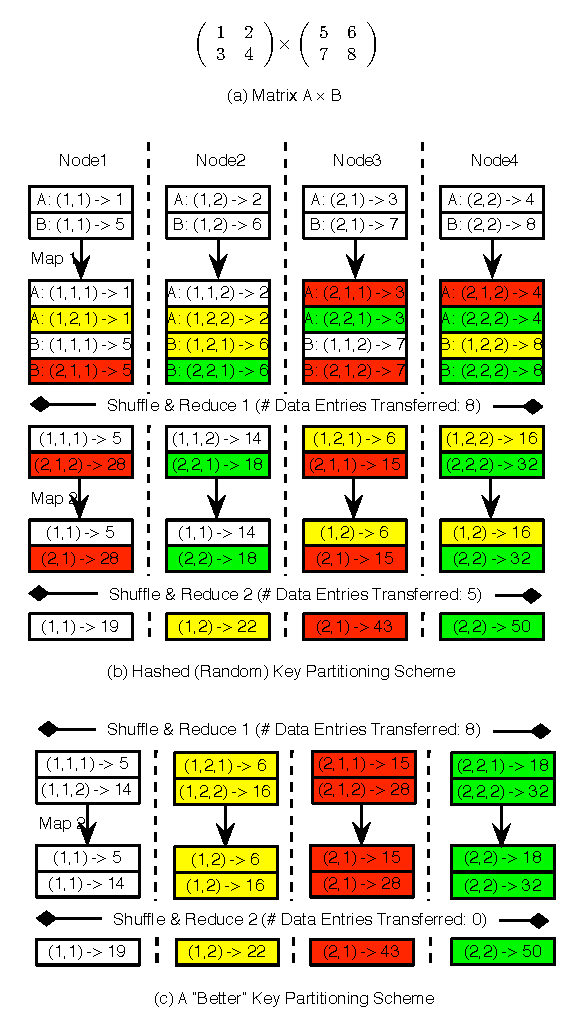
\includegraphics[width=1\columnwidth]{figure1}
\caption{An Example of the MapReduce-style Matrix Multiplication Algorithm with Different Key Partitioning Schemes 
}
\label{fig:matrixExample}
%\vspace{-0.2in}
\end{figure}



In the above simple example, obviously, there is a dependency between
the keys $(i,j,p)$ and the key $(i,j)$. Knowing and leverage this
dependency, partitioning the data entries to decrease/minimize the shuffle
would become possible.

We present a new data structure called the \emph{key dependency graph} (KDG) for this purpose.
%to extract the semantics of the computing paradigm.
The KDG is a directed acyclic graph which depicts how the keys of the
dataset entries of each iteration are generated from the previous iteration.
From the KDG, we can identify the subgraphs in which the dataset
entries with the keys in the source nodes will only generate the dataset
entries with keys in the downstream nodes. We \st{call} \red{define} such a subgraph
the \emph{pure confluence subgraph}.
Within a pure confluence subgraph, if all the dataset entries matching
the source keys are assigned to the same node, all the generated
datasets can be computed locally in the node without shuffling.

To make use of the confluence key partitioning scheme (CKP) in iterative distributed operations, 
\st{
the programs need to add the corresponding user-defined partitioner
to guide the assignment of data entries to their desired locations.
}
\red{
programmers need to construct a KDG for a distributed operation. 
Confluence automatically generates an efficient key partitioning 
scheme from the KDG. 
This user-defined key partitioning scheme guides the assignment of data entries 
to their designated nodes. 
}
Most distributed computing paradigms, such as Spark~\cite{zaharia2012resilient} and Twister~\cite{ekanayake2010twister},
provide an interface for adding a user-defined partitioner for the shuffle
operation.
By applying the CKP scheme, the shuffle sizes of multiple computing
iterations can be reduced significantly. %in polynomial time,
Note that this will not impact the computing workload skew level; that is,
the standard deviation of the computing workloads of the
nodes in the cluster after applying CKP will not be larger than that
with the random hashing scheme.
We are not aware of any previous work
%As far as we know, we are the first
that also tried to decrease the overall
shuffle traffic by a key partitioning scheme across multiple
iterations based on the
key dependency relationship.
%\textcolor{red}{Performance}

Our major contributions are listed as follows.
\begin{itemize}
\setlength{\itemsep}{0pt}
\setlength{\parskip}{0pt}
\setlength{\parsep}{0pt}
\item We invented the new data structure Key Dependency Graph to depict the iterative key dependency
and used the Confluence Key Partitioning (CKP) scheme to decrease the shuffle traffic
across distributed computing iterations.

\item We \st{gave} \red{created} the method to analyze the data transfer size and the workload skewness when using CKP, which offers the solid shuffle traffic improvement with guarantees. 

\item We implemented CKP in Spark and illustrated the use of CKP with several typical iterative distributed applications from different fields. 
The experiment on the medium-size Spark cluster demonstrates that CKP could decrease the overall shuffle traffic workload by as much as 50\%.  
\end{itemize}


The rest of the paper is organized as follows. Section~\ref{section:background}
gives some background information on iterative distributed operations
, dependency graph, and the model of the iterative shuffle size.
In Section~\ref{section:keyDependencyGraph}, we show how to construct
the KDG and to reduce effectively the shuffle sizes by the Confluence Key
Partitioning scheme, as well as analyzing the workload skew level.
Section~\ref{section:application} introduces how to apply CKP in
the real-life iterative distributed applications 
and Section~\ref{section:implement} discusses the
implementation details of CKP in Hadoop and Spark.
The evaluation results of the performance are presented in Section~\ref{section:evaluation}. 
We discuss the related work in Section~\ref{section:relatedWork} and
conclude the paper and suggest some possible future work in
Section~\ref{section:conclusion}.


\section{Background}\label{section:background}
\subsection{Iterative Distributed Operations}
Datasets of large volume cannot be stored in a single computer node
and are often separated into several partitions, 
where each partition is distributed to a node in the computer cluster. 
We refer to a dataset which is separately stored in several nodes as a distributed dataset. 
The function whose inputs include the distributed dataset is called a \emph{distributed operation}.
Each entry of the distributed dataset can be represented as a key-value pair. 
%\textcolor{red}{How to obtain each entry in the dataset. }

In many distributed computing paradigms, there are often several
iterations involving different distributed operations being applied
to the input dataset before the final results are obtained. 
Each iteration usually takes the outputs of the previous iteration as
the input dataset.

One typical example of the distributed operation is
MapReduce~\cite{dean2008mapreduce}, which divides the operation into two
primitives: map and reduce.
Many iterative distributed paradigms such as the in-memory paradigm
Spark~\cite{zaharia2012resilient} and the distributed database query
engine Hive~\cite{thusoo2009hive} can be equated to multiple
iterations of MapReduce operations.
For iterative distributed
operations, we refer to the general iterative map-and-reduce operation, 
where the ``map'' primitive performs one or more transformation operations on the
datasets in each local node, and the ``reduce'' primitive would
re-partition the datasets by transferring the data entries with
the same keys to the designated locations and group the entries of the same key to one key-value pair, where this \textit{value} is a list of the values that associate with the key. 
The output of each data entry of the reduce primitive is also called as the key-value-list pair in this paper.
The reduce primitive does not involve any transformation on the values of the entries and is also known as the shuffle operation. 

Note that division of map and reduce in the matrix multiplication example in Section~\ref{section:introduction} is slightly different from the definition here. 
In the example, the reduce primitive aggregate the value list of each key to a value, which follows the traditional style of MapReduce. 
While by the definition here, the aggregate operations join the other data transformation operation in the map primitive of the next iteration. 
Each iteration of distributed operation can have a series of transformations plus at most one shuffle operation.
In the rest of this paper, the terms of the reduce primitive and the shuffle operation may be used interchangeably. 


The traffic pattern of the data to shuffle in each iteration is directly
dictated by the key partitioning scheme.
A random or careless key partitioning scheme may cause unnecessary
shuffle traffic across multiple iterations of distributed operation.
This is what we set out to reduce using our partitioning scheme.


\subsection{Dependency Graph}
The dependency graph is a directed graph usually used for
describing the dependency relationship of instructions, tasks, data, etc
\cite{sakellariou2004hybrid,zhao2006scheduling,isard2007dryad}.
The scheduler can use the dependency graph to decide the order the execution of instructions or tasks. 
In distributed frameworks, the scheduler uses the data dependency graph
or task dependency graph to make the tasks execute in parallel in the
cluster.
As the tasks are meant to process their specific data, the task dependency
graph is the data dependency graph as well.

In the data dependency graph, the datasets are divided into graph nodes
based on locations and the dependency relationship is
constructed upon the execution stages and data locations.
The data partition information is specific to the application running
situation and the cluster environment.
In the key dependency graph proposed in this paper, the construction of
the graph does not use any data partitioning information, but considers
the key dependency of data, which depends on the
application logic.

\subsection{Iterative Shuffle Size}\label{section:model}
We model the overall shuffle size of the iterative
distributed operations and discuss the time complexity of obtaining
the optimal key partitioning scheme that minimizes the overall shuffle
size.



For the iterative distributed operations, the result of the $i_{th}$ iteration can be obtained recursively by:
\begin{equation}\label{eq:m}
A'_i=m_i(A_{i-1})
\end{equation}
\begin{equation}\label{eq:r}
A_i=r_i(A'_i)
\end{equation}
, where $A_{i-1}$ is the output of the $(i-1)_{th}$ iteration as well as the input of the $i_{th}$ iteration, 
$m_i$ is the map primitive of the $i_{th}$ iteration that operates on $A_{i-1}$ locally without changing the partition locality, 
and $r_i$ is the shuffle operation of the $i_{th}$ iteration that takes the output $A'_i$ of the map primitive as the input.  
The keys of $A_i$ and $A'_i$ are the same, but the partition localities are different. 
In the first iteration, when i is equal to 1, 
$A_0$ represents the raw input datasets before any processing.  

Suppose in the $i_{th}$ iteration of the shuffle operation, in order to collect an entry $a \in A_i$, 
the size of data that need to be transferred is a function of $a$ and $A'_i$: $s_i(a,A'_i)$. The function $s_i$ can be different in different key partitioning schemes. 
The data transfer size to obtain $A_i$ is: 
\begin{equation}\label{eq:si}
\begin{aligned}
S_i&=\sum_{a \in A_i} s_i(a,A'_i).
% &=|A_i| \cdot s_i(a_i, A_{i-1})
\end{aligned}
\end{equation}

Within the same $i_{th}$ iteration, for $\forall a_p, a_q \in A_i$ where $a_p \neq a_q$, the values of $s_i(a_p,A'_i)$ and $s_i(a_q,A'_i)$ are independent of each other. 
It means that if the value of $s_i(a_p,A'_i)$ changes due to a different partition location of $a_p$, the value of $s_i(a_q,A'_i)$ remains unchanged unless $a_q$ is partitioned to a different location. 

If $m$ iterations are required to compute the final result, 
the overall accumulated data transfer size for obtaining the final result is
\begin{equation}\label{eq:s}
S=\sum_{i=1}^{m} S_i=\sum_{i=1}^{m} \sum_{a_i \in A_i} s_i(a,A'_i).
\end{equation}


If values of $S_i (1 \leq i \leq m)$ are independent of each other, 
$S$ is a linear function and $S$ can be minimized simply by minimizing each $s_i(a,A'_i)$.
However, most usually, $S_i$ and $S_{i+1}$ are correlated.
The value of $S_i$ depends on the logic of the function $m_i$ in Formula \ref{eq:m}, 
the partition locality of dataset $ A_{i-1}$, 
as well as the locations where each entry of $A_i$ is partitioned to. 
The partition locality of $A_i$ inherited from the $i_{th}$ iteration 
will again affect the value of $S_{i+1}$.
%\textcolor{red}{add Markov-Chain-like relation here}

If the contents of $A_i (i=1,2,...,m)$ are already known, to find out the optimal key partitioning scheme that minimizes 
%A clumsy and straightforward way to minimize 
the overall data transfer size $S$,  %is 
we need to exhaustively explore the possible key partition schemes of all the key-value pairs across all the iterations. 
By calculating the overall data transfer size of each scheme, the optimal solution is the scheme with the minimal size. 
The time complexity of the exhaustive method is $O(n^{\sum_{i=1}^{m} |A_i|}$), 
where $n$ is the number of nodes in the cluster and $|A_i|$ is the number of data entries of $A_i$, 
which indicates that it is an NP-complete problem. 

In fact, we usually do not know the contents of $A_i$ and cannot explore the partition scheme 
for the next iteration until the program has actually finished the $i_{th}$ iteration. 
Due to this limitation, the idea of finding out the optimal partition schemes for all the iterations to minimize the overall data transfer size $S$ is infeasible. 
In the rest of this paper, the shuffle size is used to refer to the data transfer size of the shuffle operation. 


\section{Confluence}\label{section:keyDependencyGraph}
Even though it is hard to find the optimal partition solution to minimize the overall shuffle size,
if the code logic of the specific distributed operations is already known, 
the shuffle size can be reduced to the maximum extent %in polynomial time 
by exploring the key dependency of different iterations. 

This section firstly describes the the construction process of the key dependency graphs, as well as its properties. 
After that, we present Confluence Key Partitioning Scheme, which decreases the overall iterative shuffle size by applying the properties of the key dependency graph, while not increasing the workload skew level. 


\subsection{Key Dependency}\label{section:dependency}
Given a key-value pair as the input to an iteration of the distributed operation,
it will generate a (or a set of) new key-value pair(s) based on the logic of the program. 
The distributed key dependency
represents such logic of the generation of key-value pairs from the input key-value pairs in every iteration
of the distributed operation. 
The programmer is supposed to be well acquainted with the distributed operation logic. 
By saying that we know the key dependency for a specific iterative distributed operation,
it means that we know what the output key-value pairs will be 
for an input key-value pair in every computing iteration. 
We use the key dependency graph (introduced later) to portrait the iterative key dependency
so that it is comprehensible to the computer. 
Every distributed operation has its own key dependency
and it relies on the programmer to understand the iterative key dependency based on the application logic
and construct the key dependency graph.


\begin{figure}[!t]
\removelatexerror

\begin{algorithm}[H]
\SetKwInOut{Input}{Input}
\SetKwInOut{Output}{Output}

 \Input{Key Set $K_i$, containing all the possible keys (or usually, key patterns) of the output key-value pairs of any Iteration $i$;\\
 Key Dependency Set $D$, containing the key dependency of all iterations;
 }
 \Output{Key Dependency Graph $G=(V,E)$}
\tcc{Construction of $V$}
 \ForEach{Iterations $i$}{
  \ForEach{$k \in K_i$}{
    add vertex $v_{i,k}$ to $V$
  }
  \If{any possible key (key pattern) is unknown}{
    add vertex $v_{i,x}$ to $V$
  }
}

\tcc{Construction of E}
\ForEach{Iterations $i$}{
  \ForEach{key dependency $v_{i,k1} \Rightarrow v_{i+1,k2}$ in $D$}{
    add edge $(v_{i,k1}, v_{i+1,k2})$ to $E$
  }
}
\caption{Construction of the Key Dependency Graph}
\label{algo:KDG}
\end{algorithm}

\caption{Pseudo Code of Constructing the Key Dependency Graph}
\label{fig:KDG}
\end{figure}


\subsection{Key Dependency Graph}\label{section:kdg}

The directed graph $G=(V,E)$, which is named as the \emph{key dependency graph} (KDG), addresses the key dependency status of the distributed operation iterations. 

The key pattern is the symbol that represents a set of keys that match a specific pattern.
The key dependency is denoted with two vertexes $v_{i,k1} \Rightarrow v_{i+1,k2}$ if
the output key-value pairs with key matching pattern $k1$
in Iteration $i$ can generate a key-value pair with key matching pattern $k2$ in Iteration $i+1$.
The key dependency is specific to the code logic of the distributed operation 
and it decides which graph node should point to which others. 
The distributed operation code logic should be known prior by the programmers.

The construction process of the key dependency graph G is shown as in Algorithm~\ref{algo:KDG}.
Note that when constructing $E$, for the unknown keys (or key patterns), it is assumed that $v_{i,x} \Rightarrow v_{i+1,k2}, \forall k2$. 
The unknown key dependency is only raised when there are some key values (or key patterns) the programmer cannot make sure in a computing iteration. 
In practice, the input set $K_i$ in Algorithm~\ref{algo:KDG} is defined to contain the key patterns instead of the distinguished key values, so that a node in the KDG represents a key pattern. 
Such practice limits the width of the KDG in each level
and our algorithm introduced later can partition the key-value pairs based on their key pattern. 
In the rest of this paper, unless specified, the input set $K_i$ is the key pattern set, 
but for generality, we still refer to it as the key set. 

%The construction of the KDG $G=(V,E)$ is finished here. 
This graph is a directed acyclic graph (DAG).
The time complexity to construct this graph is $O(\sum_{i=1}^m k_{i-1} k_i)$, 
where $k_i$ is the number of keys (or key patterns) in iteration i and $m$ is the total number of iterations.
Usually, $k_i$ is very small in value when it is referred as the key pattern (not the distinguished values of the keys).
For example, in the matrix multiplication application, the subgraph from the second level to the third (final level) of the KDG can be denoted as a one node to one node subgraph: $(a, b, [1, n]) \rightarrow (a, b)$, 
where $a$ and $b$ stand for any row and any column index of the matrix, 
and $[1, n]$ stands for the range from 1 to the the matrix dimension length $n$.

The subgraph $C=(V', E')$ of $G=(V,E)$ is called a \emph{confluence subgraph} if it satisfies the following
\emph{outward exclusive} requirements: 
denote $V'_i$ as the set of all the vertexes in $V'$ which are in level $i$ in $G$.  
$V'_i$ satisfies $V'_i=\bigcup_{v'_{i-1} \in V'_{i-1}}V_i$, where $V_i$ is the set of vertexes that $v'_{i-1}$ has an edge $e \in E$ points to. 
%For any $v'_1 \in V', v'_2 \in V'$, if $e' =(v'_1,v'_2) \in E$, 
%then $e' \in E'$. For any $e'=(v'_1,v'_2)\in E'$, $v'_1 \in V'$ and $v'_2 \in V'$. 
The edge $e' =(v'_1,v'_2)$ is in $E'$ iff $v'_1 \in V', v'_2 \in V'$ and $(v'_1,v'_2) \in E$.

In other words, in the confluence subgraph, all the vertexes in the upper level have no edge pointing to
the vertexes in the lower level outside the confluence subgraph. 
Let Level $u$ and Level $w$ be the uppermost level and the lowest level that $V'$ contains, respectively. 
$V'_u$ is called the \emph{source key set} at level $u$ and $V'_w$ the \emph{confluence key set} at level $w$
of the confluence subgraph $C=(V',E')$. 

We call the confluence subgraph $C=(V', E')$ the \emph{pure confluence subgraph} if 
it further satisfies the \emph{inward exclusive} requirement: 
$V'_{i-1}=\bigcup_{v'_i \in V'_i}V''_{i-1}$, where $V''_{i-1}$ is the set of vertexes that have an edge $e \in E$ pointing to $v'_i$. 

%\textcolor{red}{the time complexity of getting the confluence subgraph}

An example of the KDG of 3 levels and some of its confluence subgraphs are shown in Fig.~\ref{fig:keyDependencyGraph}. The subgraph in the dashed boxes C3 is a pure confluence subgraph 
of C1. The subgraph in C2 is a confluence subgraph but not a pure confluence subgraph, 
as the source node of the edges $(v0x, v11)$ and $(v0x, v12)$ is not in C2. 
The subgraph in the dotted box C4 is not a confluence subgraph as the edge $(v0x, v12)$ 
points to the node $v12$, which is not a vertex in the subgraph C4. 
Note that the key dependency graph is always the pure confluence subgraph of itself, as show in the dashed box C1. 

\begin{figure}[!t]
\centering
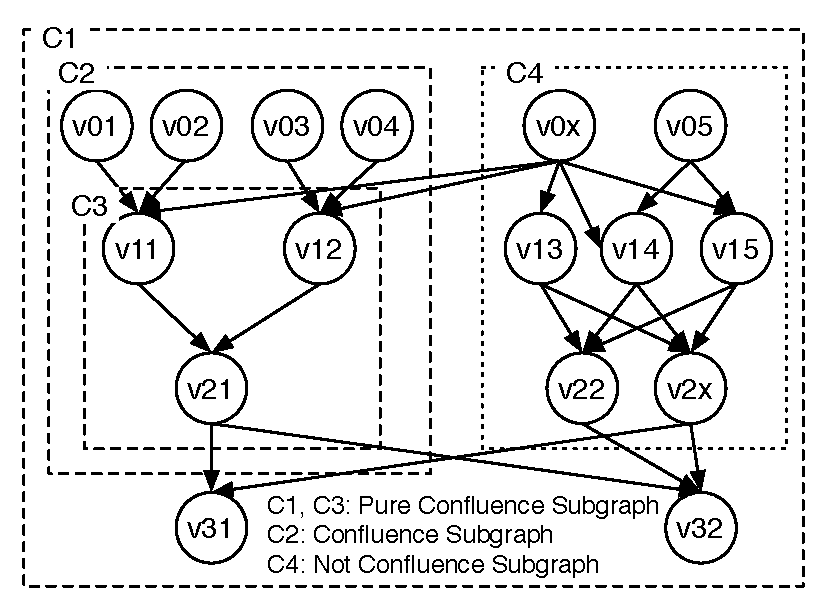
\includegraphics[width=1\columnwidth]{figure3}
\caption{A Key Dependency Graph Example}
\label{fig:keyDependencyGraph}
%\vspace{-0.2in}
\end{figure}

\subsection{Properties of Confluence Subgraph}
For the distributed operations of several iterations, suppose that there is a confluence subgraph $C$ of its KDG 
with the source key set $V'_u$ at level $u$ and the confluence key set $V'_w$ at level $w(w > u)$. 
Let $B_u$ be a part of the output dataset of the $u_{th}$ iteration 
and $B_w$ be the dataset generated by $B_u$ after $(w-u)$ iterations. 
%Let $A_u$ and $A_w$ be a part of the output datasets of the $u_{th}$ and $w_{th}$ iteration, respectively.
We have a theorem that can easily be conducted by the definition of the confluence subgraph. 

\newtheorem{theorem}{\textbf{Theorem}}
\begin{theorem}\label{thm:upwardClosure}
If the keys of all the entries of $B_u$ are in the source key set $V'_u$, 
the keys of all entries of $B_w$ are in the confluence key set $V'_w$. 
\end{theorem}

We call the datasets $B_u$ and $B_w$ in Theorem \ref{thm:upwardClosure} 
the \emph{upward closure pair} datasets of the confluence subgraph. 
It can be further conducted from Theorem \ref{thm:upwardClosure} to get:

\newtheorem{conduction}{\textbf{Theorem}}[theorem] 
\begin{conduction}\label{thm:zeroTransfer}
If the subgraph $C$ is a pure confluence subgraph and the keys of all the entries of $B_u$ are in the source key set $V'_u$, 
when $B_u$ is stored in one single node, 
the minimum data transfer size for obtaining $B_w$ is 0. 
\end{conduction}

Theorem \ref{thm:zeroTransfer} indicates that if the datasets $B_u$ and $B_w$ are 
the upward closure pair of a pure confluence subgraph 
and $B_u$ is partitioned in one node, 
we can finish all the following $(w-u)$ iterations of distributed operations in the same node to obtain $A_w$, 
without any data transferring. 
We name this key partitioning scheme the \textbf{Confluence Key Partitioning} scheme. 


%\textcolor{red}{The usage of the confluence keys}
%\textcolor{red}{how it reduce the data transfer size}
\subsection{Confluence Key Partitioning}\label{section:CKP}
We demonstrate that the overall data transfer size can be decreased by 
localizing the pure confluence subgraph, 
i.e., placing the datasets corresponding to the pure confluence subgraph in a node. 

Assume that there is a pure confluence subgraph $C$ in the KDG, 
from level $u$ to level $w(u \neq 0, w>u)$. 
Let $V'_u$ and $V'_w$ be the source key set and the confluence key set of $C$, respectively, and $B_u$ and $B_w$ be the upward closure pair datasets. 
The \emph{Confluence Key Partitioning (CKP)} scheme partitions the dataset $B_u$ %, whose keys are all in $V'_u$, 
in one single node in Iteration $u$
and completes the following $(w-u)$ iterations of operations on $B_u$ and its generated dataset in the same node. 

CKP localizes the data in the granularity of a pure confluence subgraph, different pure confluence subgraphs are partitioned randomly. 

Although the KDG is the pure confluence subgraph of itself,
we do not consider the localizing the whole KDG in the above discussion. 
The reason is that the raw input dataset %which is considered as the output of iteration 0
is always distributed across the cluster before the first iteration. 

We analyze the expected overall data transfer size $S'$ of CKP
in comparison with that $S''$ of the random key partitioning scheme (RKP), which is ignorant of the key dependency and partition the data entries randomly (e.g., partition by the hashed value of keys). 
$S'_i$ and $S''_i$ denote the expected data transfer size of CKP and and RKP in the $i_{th}$ iteration, respectively.  
% We assume that in every iteration, each key is expected 

Before going further, we figure out the function $s_i(a,A'_i)$ in Formula \ref{eq:si} in the case that $a$ is randomly (uniformly) partitioned to a node. 
In this case, the probability of $a$ is partitioned to any node is $1/n$, where $n$ is the number of nodes in the cluster. 
We call such an entry that has the same probability being partitioned to any node as the uniformly-partitioned entry. 
As long as the partition location of an entry is finally hashed to the computer nodes, the entry is a uniformly-partitioned entry.

Suppose that $a'$ is the set of input data entries that have the same key as $a$ right before the shuffle operation and $p_j$ denotes the percentage of data entries of $a'$ that lie in Node $j$, where $\sum_{j=1}^{n} p_i=1$.
We have
\begin{equation}\label{eq:si2}
s_i(a,A'_i)= \sum_{j=1}^{n} [\frac{1}{n}|a|(1-p_j)]=\frac{(n-1)} {n}\cdot |a|
\end{equation}
, where $|a|$ is the length of the value list of $a$, which is also the number of data entries in $a'$. 
It shows that if $a$ is randomly partitioned to a node, 
the distribution of $a'$ does not affect the data transfer size for collecting $a$. 

\newtheorem{siTheorem}{\textbf{Theorem}}
\begin{theorem}\label{thm:siTheorem}
The data transfer size for collecting the uniformly-partitioned entry in the shuffle operation is decided only by the number of nodes in the cluster and the length of this entry. 
\end{theorem}

By Theorem \ref{thm:siTheorem}, when using RKP, the data transfer size of the $i_{th}$ iteration is $S''_i=\sum_{a\in A_i} \frac{(n-1) \cdot |a|}{n}=\frac{n-1}{n}|A'_i|$, 
where $|A'_i|$ is the number of data entries in $A'_i$.

For CKP, we analyze every iteration as follows. 

\begin{itemize}
\setlength{\itemsep}{0pt}
\setlength{\parskip}{0pt}
\setlength{\parsep}{0pt}
\item[1)] From Iteration $1$ to $(u-1)$, the key partitioning scheme is the same as RKP: 
$S'_i=S''_i, 1 \leq i \leq u-1$. 

\item[2)] In Iteration u, an entry of $B_u$ belongs to a pure confluence subgraph and the pure confluence subgraph is randomly partitioned. 
The entries in $B_u$ are uniformly-partitioned entries, as well as the entries in $A_u-B_u$. Therefore, $S'_u=S''_u$.

\item[3)] From the $(u+1)_{th}$ to $w_{th}$ iteration, the data transfer size of the operations on the datasets generated by $B_u$
is 0, by Theorem \ref{thm:zeroTransfer}. 
We have $S'_i=S''_i-\frac{n-1}{n}|B'_i|$, 
where $r_i(B'_i)=B_i, u+1 \leq i \leq w$. 

\item[4)] From iteration $(w+1)$ onward, the data entries are uniformly-partitioned entries again:
$S'_i=S''_i, i \geq w+1$.
\end{itemize}

In all, the expected overall data transfer size after applying CKP 
is $S'=S''- \frac{n-1}{n}\sum_{i=u+1}^w |B'_i|$, 
which eliminates exactly the shuffle workload of the datasets that associate with the keys in the pure confluence subgraphs as compared to RKP, without introducing other shuffle workloads. 
$\sum_{i=u+1}^w |B'_i|$ stands for the shuffle size improvement of CKP as compared to RKP.
This result indicates that CKP can reduce more data transfer size 
if the pure confluence subgraph contains more iterations 
or the size of the dataset corresponding to the pure confluence subgraph is larger. 
In Section~\ref{section:application}, the value of $\sum_{i=u+1}^w |B'_i|$ will be figured out for the specific distributed operations.


\subsection{Workload Skew Analysis}\label{section:skew}
The workload of a node is the number of data entries of the map primitive in that node and 
The workload skew level of Iteration $i$ is the standard deviation of the expected workloads of different nodes in that iteration, which is denoted as $L_i$. 
The math symbols in Section~\ref{section:CKP} are reused here without duplicated definition. 
Only the data entries that associate with the pure confluence subgraphs are counted as the other data (if any) are randomly partitioned in both RKP and CKP and will not affect the standard deviation of the workloads.
And we only consider the workload skew levels of the iterations that the pure confluence subgraphs affects (Iteration $u+1$ to $w+1$).
The reason is that both RKP and CKP use the same key partitioning policy in the CKP-not-affected iterations and the workload skew levels of these iterations will be the same in both schemes.


In all iterations when RKP is applied, every entry is a uniformly-partitioned entry, the expected workloads of the all the nodes are the same and the expected workload skew level is 0. 

When CKP is applied, as each output entry of the shuffle operation is the uniformly-partitioned entry in Iteration $u$, the workloads of all the nodes are the same in Iteration $u+1$. 
Therefore, $L_{u+1}=0$.

In Iterations from $u+2$ to $w+1$, 
it can be divided into two phases based on the \st{semantics} logic of the distributed operations. 
Suppose that Iteration $u' (u+1 \leq u' \leq w)$ is such an iteration that in every iteration from $u+1$ to $u'-1$, each input entry of the map primitive is expected to generate the same number of output entries of the shuffle operation, and in Iteration $u'$, the expected number of output entries of the shuffle operation generated by each map input entry is unknown or not the same. 
Note that such Iteration $u'$ may not exist and in this case, we denote it as $u'=w+1$. 

\textbf{Phase 1}: From Iteration $u+2$ to $u'$, 
the workloads are the same in all the nodes and the workload skew level of every iteration is 0.

\textbf{Phase 2}: From Iteration $u'+1$ to $w+1$, 
the workloads of the nodes in each iteration are unpredictable, 
which are dependent on the number of data entries that can be generated by the data localized in each node. Therefore, $L_i \geq 0, u'+1 \leq i \leq w+1$.

Although the workload skew levels of CKP in Phase 2 is unpredictable,
fortunately, such Iteration $u'$ does not exist in many distributed operation, 
including matrix multiplication and the other distributed applications (MovieLensALS, MultiAdjacentList and KMeans) introduced in Section~\ref{section:application}. 
In these applications, the expected workload skew level of CkP is 0, which is the same as that of RKP.
In the distributed application where $u'$ does exist, the workload skew level may not be 0 and specific workload skew analysis is needed for this specific application.


\subsection{Affect of Inaccurate KDG}
Note that the programmers do not need to change the original logic of programs 
in order to apply CKP. 
A wrong or inaccurate KDG will not impact the accuracy of the computation results, but only affect results of key partitioning locations. 
Unpredictable workload skewness may exist, but as CKP randomly partitions the pure confluence subgraphs, the workloads tend to be balanced in all the nodes. 



%\textcolor{red}{TODO}

%Matrix Multiplication
\section{Application}\label{section:application}
% In this section, we illustrate how CKP can be applied to the matrix multiplication algorithm straightforwardly. 
In this section, we show how CKP can be applied in various
iterative distributed applications, even when the applications are not well-structured and the pure confluence subgraphs
are not obvious, by dividing the operations into multiple sub-operations.

In the key dependency graph of the matrix multiplication algorithm, 
the pure confluence subgraphs are obvious in the second iteration, 
whose keys follow the many-to-one mapping pattern.
In some cases, CKP may not be applicable when
the pure confluence subgraphs cannot be found
%for the whole iterative distributed operations
in the straightforward way.
In this case, if the iterative distributed operations can be divided into several smaller operations to fit the Confluence model, 
CKP can be flexibly applied to some of the divided operations.
The division of the iterative distributed operations can be based on either the operations or the datasets. 
In the following, we illustrate the methods to divide the iterative
distributed operations with the real-life application examples, 
namely MovieLensALS, MultiAdjacentList and KMeans.




\begin{figure*}[!t]
\centering
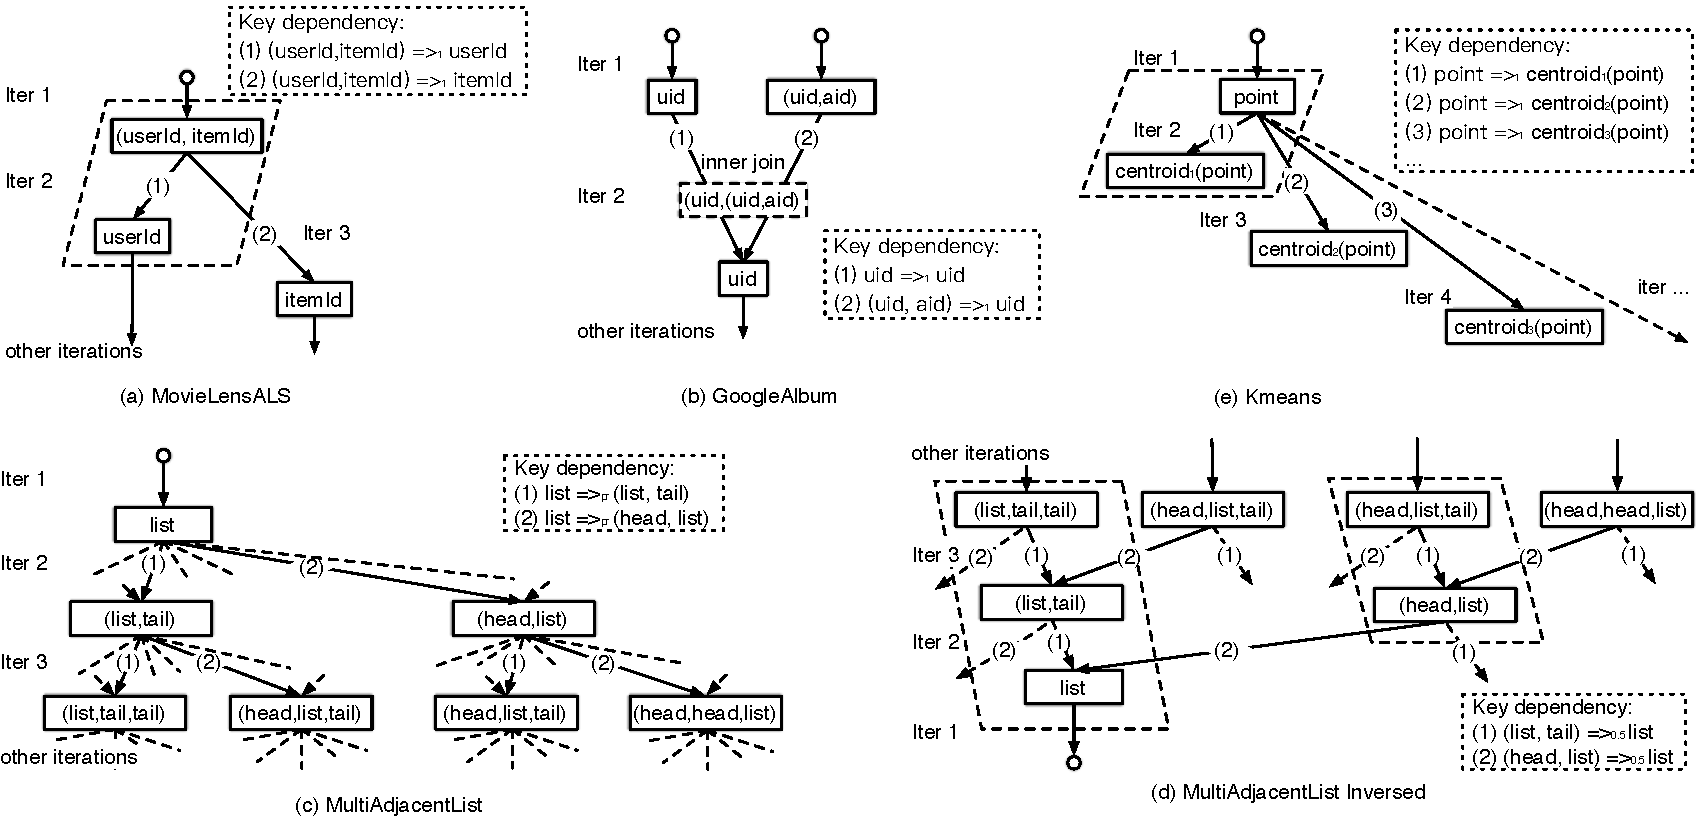
\includegraphics[width=2\columnwidth]{figure4}
\caption{The Original (Suffixed by \_O) and Divided (Suffixed by \_D) Iterative Evolution of the Datasets of the MovieLensALS and MultiAdjacentList Applications. The Keys of the Datasets are Marked by Parenthesis. Pure Confluence Subgraphs can be Found in the Computing Iterations in the Dashed Boxes
}
\label{fig:alsDivision}
%\vspace{-0.2in}
\end{figure*}


\subsection{MovieLensALS}
MovieLensALS \cite{movielensals} is a
recommendation application that uses Alternating Least Squares (ALS)
method in collaborative filtering in order to recommend the product
items to the users based on the user-item rating information.
During the execution, it organizes the rating data into the user-item
blocks grouped by the keys ``$(userId, itemId)$".
In the successive iterations, it needs to reorganize the user-item block
data by generating the user block and the item block grouped by
``$userId$'' and ``$itemId$'', respectively.
This operation is done in two iterations as shown in Fig.~\ref{fig:alsDivision}(a). 
No single key partitioning scheme can remove the shuffle data in order
to generate both of these blocks from the user-item block, as the key
dependency follows a many-to-many pattern.
However, if the programmer regards the iterative distributed operation as two
individual iterative operations and the operation is divided as in
Fig.~\ref{fig:alsDivision}(b), the pure confluence subgraph can be found in
the operation in the dashed box.
CKP can then be applied on the key dependency $(userId, itemId) \Rightarrow
userId$ for the user block.

As CKP is applied only in one successive iteration in MovieLensALS, the workload skew level is 0.

\begin{table}[!t]
% increase table row spacing, adjust to taste
\renewcommand{\arraystretch}{1}
% \extrarowheight as needed to properly center the text within the cells
\caption{CKP Shuffle Size Improvements in Different Distributed Operations}\label{table:skew}
\centering
% Some packages, such as MDW tools, offer better commands for making tables
% than the plain LaTeX2e tabular which is used here.
%\begin{tabular}{|c||c|c|}
\begin{tabularx}{0.5\textwidth}{ c || c }
\hline
\textbf{Distributed Operations} & \textbf{CKP Shuffle Size Improvement}  \\
\hline
MatrixMultiplication & $n^3 for R^{n \times n}$\\
\hline
MovieLensALS  & \# of $(user,item)$ entries  \\%; input file size 640 MB 
\hline
MultiAdjacentList  & 1/2 the RKP shuffle size in every iteration \\
\hline
KMeans & $|A| \cdot \sum_{i=2}^{m} (\sum_{j=1}^{k} p'_{ij} - 1/n)$ \cr
& upper bound:$|A| \cdot (m-1)(n-1)/n$ \cr
& lower bound:$-|A|\cdot (m-1)/n$\\
\hline
\end{tabularx}
%\end{tabular}
\end{table}



\subsection{MultiAdjacentList}
MultiAdjacentList \cite{multiAdjList} is
a graph computing application which generates the heads and tails of
lists of various lengths from the information of edges.
In every iteration, where the key $L_i$ represents a list of length $i$ and its values are the sets of the head nodes and tail nodes of the list, it
generates a group of new lists of length $i+1$ by appending each head
node and each tail node to it. Each new list acts as the key and
its new head nodes and tail nodes act as the value.
The evolution of the data of multiple iterations is shown as Fig.~\ref{fig:alsDivision}(c).
The key dependencies are $L_i \Rightarrow (heads, L_i)$ and $L_i \Rightarrow (L_i, tails)$. 
We cannot use CKP to localize the keys $(heads, L_i)$ and $(L_i, tails)$ with $L_i$, 
as the datasets corresponding to Key $(heads, L_i)$ and Key $(L'_i, tails)$ may overlap for different $L_i$ and $L'_i$.
However, the programmer can divide the iterative operations into several smaller iterative operations by dividing the dataset as in Fig.~\ref{fig:alsDivision}(d). 
In the iterative operations in the dashed boxes, the pure confluence subgraphs exist 
in their KDG's by the key dependency $L_i \Rightarrow (L_i, tails)$.
Applying CKP to these operations and leaving the other iterative operations
that are related to the keys $(heads, L_i)$ to be randomly partitioned,
only half of the datasets need to be shuffled. 

In the setting that every node has $l$ heads and $l$ tails on average, every map input entry is expected to generate $2 \cdot l$ shuffle output entries in each iteration. Therefore, by the discussion in Section~\ref{section:skew}, the workload skew level of each iteration is 0 when CKP is applied. 

\subsection{KMeans}
KMeans \cite{kmeans} is the popular clustering algorithm in data mining, which groups the vector points into $k$ clusters where each vector point belongs to the cluster with the nearest mean. 
This process could be done in a dedicated number of iterations. 
With the initial $k$ chosen points regarded as the centers of the clusters, 
in each iteration, every point is compared with the $k$ centers and is is grouped into the cluster where the Euclidean distance between the point and the center is the smallest. 
After all points are grouped, each new cluster center for the next iteration is chosen by the mean of the points in that cluster. 
The shuffle operation takes place when calculating the mean of each cluster whose points are located in different nodes. 

If the points are bound to the same cluster in every iteration, 
by using the key dependency $points \Rightarrow centers$ 
and localizing the points in the same cluster at the first iteration, 
CKP can eliminate the shuffle size in the successive iterations. 
However, the affiliation of point to clusters are not stable between iterations. 
One point that is grouped into one cluster in a iteration can be grouped into another cluster in the next iteration. 
We estimate the shuffle size in this case. 

Suppose that $p'_{ij}$ is the percentage of points that are grouped in Cluster $j$ both in the first CKP iteration and Iteration $i (i \neq 1)$, 
$|A|$ is the total number of points, $m$ is the total number of iterations, 
and $n$ is number of nodes. 
The shuffle size of Iteration $i$ is $S_i=|A| \cdot (1-\sum_{j=1}^{k} p'_{ij})$.
The CKP shuffle size improvement in Iteration $i$ is 
$(n-1)/n \cdot |A| - S_i = |A| \cdot (\sum_{j=1}^{k} p'_{ij} - 1/n)$, 
and the overall CKP shuffle size improvement is $|A| \cdot \sum_{i=2}^{m} (\sum_{j=1}^{k} p'_{ij} - 1/n)$.
The higher $\sum_{i=2}^{m} \sum_{j=1}^{k} p'_{ij}$ is, the higher the shuffle size improvement. 
In the best case that points are bound to the same cluster in every iteration, 
$\sum_{j=1}^{k} p'_{ij}=1 (i=2,3,...m)$ 
and the shuffle size improvement is $|A| \cdot (m-1)(n-1)/n$.
In the worst case, every point grouped into cluster $i$ in the first iteration is grouped to a cluster other than $i$, the shuffle size improvement is 
$-|A|\cdot (m-1)/n$. 
The affiliation of the points to the clusters are more stable after running a few iterations. 
Instead of localizing the points of the same cluster in the very first iteration of KMeans, localizing them after a few beginning iterations can give higher $\sum_{j=1}^{k} p'_{ij}$.

In every iteration of KMeans, as every input point generates the same point as the input for the next iteration, the workload skew level of every iteration is 0. 


A summary of the CKP shuffle size improvements of the distributed operations discussed above is shown in Table~\ref{table:skew}.
All the values of the CKP shuffle size improvement are figured out without consideration to the map-side combine mechanism discussed in Section~\ref{section:implement}.


\begin{table*}[!t]
\begin{threeparttable}[b]
% increase table row spacing, adjust to taste
\renewcommand{\arraystretch}{1}
% \extrarowheight as needed to properly center the text within the cells
\caption{User-Defined Functions of ConfluencePartitioner in Different Distributed Operations}
\label{table:code}
\centering
% Some packages, such as MDW tools, offer better commands for making tables
% than the plain LaTeX2e tabular which is used here.
%\begin{tabular}{|c||c|c|}
\begin{tabularx}{0.98\textwidth}{ c || c |c  }
\hline
\textbf{Distributed Operations} & \textbf{Key Dependency} & \textbf{User-Defined Function} \\
\hline
MatrixMultiplication & $(i,j,p) \Rightarrow (i,j)$ & (a:Any) $=>$ a match \{case (\_ , \_, \_) $=>$ (a.\_1, a.\_2)\}\\
\hline
MovieLensALS  &$(user,item) \Rightarrow user$ & (a:Any) $=>$ a match \{case (\_ , \_) $=>$ a.\_1\} \\%; input file size 640 MB 
\hline
MultiAdjacentList  & $list \Rightarrow (list, tails)$ & (a:Any) $=>$ a match \{case s:String $=>$ \{s.split(" ")(0) \}\}\\
\hline
KMeans & $points \Rightarrow cluster$ & (a:Any) $=>$ a match \{case point:Vector[Double] $=>$ closestPoint(point, cluster\_centers)\tnote{1}\\
\hline
\end{tabularx}
%\end{tabular}
\begin{tablenotes}
    \item[1] closestPoint(point, cluster\_centers) is the function which returns the index of the point in ``cluster\_centers'' that is in the shortest Euclidean distance with ``point''. The ``cluster\_centers'' are the cluster centers of a fixed iteration, e.g., the first iteration. 
  \end{tablenotes}
\end{threeparttable}
\end{table*}

\section{Implementation}\label{section:implement}
This section introduces the effect of the map-side combine mechanism and the
limitations of applying CKP in MapReduce.
The implementation details of binding partitions and executors to
facilitate CKP in Spark and the discussion on how to automate
the confluence approach will also be presented.

\subsection{Map-Side Combine}
In practice, existing distributed frameworks can do map-side
combine for the map output data before the shuffle operation if the
reduce operation is an aggregate function, e.g, the sum function of the
reduce operation in Stage 2 of the matrix multiplication algorithm as
mentioned above.
The map-side combine does the local reduce operation on map output data
such that the data needed to transfer in the shuffle operation can be
greatly decreased in size even when RKP is applied.
However, CKP is still beneficial because it eliminates the overhead time
of initializing and cleaning up the %bunches of
shuffle connections, which can be time-consuming.


\subsection{Confluence in Hadoop}
CKP can be widely applied to decrease the shuffle size of the iterative
distributed paradigms that compute and store intermediate datasets in
the memory, like Spark and Twister.
However, we find it not applicable to Hadoop MapReduce for the following reason. 
Hadoop MapReduce stores the output result of each distributed operation
iteration in the distributed file system, i.e., HDFS,
where the partitioned locations of the data blocks are reorganized due to the internal storing mechanism of HDFS.
Even if the datasets are partitioned by CKP during the distributed
operation, the partitioned locations of the datasets will not be
retained in the next iteration of the distributed operation.

An alternative solution is to modify the mechanism of HDFS on choosing the
partitioned locations of data blocks when storing data to a file.
If the dataset is able to declare the preferred partitioned location as the node where it is kept in the memory and HDFS writes the dataset to its preferred partitioned locations, the partitioned locations of the datasets will remain unchanged and CKP is applicable. 
We have not implemented this new mechanism in HDFS and the feasibility is yet to be verified. 


\subsection{Binding Partition and Executor in Spark}
In the implementation of Spark, the partition is only a logical location where the task executes the dataset, while the logical locations of tasks are not tied up with the actual(physical) positions of the executors. 
In other words, %if a dataset is assigned to the same partition, 
the tasks working on the same partition are not guaranteed to be assigned to the same executor (or the same computer node) across different iterations, in which case shuffling of data is still needed. 

To amend the mismatch of the logical partition and the actual position of the executor, we implement the new feature in Spark to allow the binding of the task partitions and the executors. 
The binding can be done in the hash manner. 
In the default settings of the task scheduler of Spark, when an executor becomes free, the task scheduler selects the task with whichever partition from the head of task queue. The selected task will run in that executor. 
Now, if the partition-executor-binding feature is turn on, when the task scheduler selects a task for the free executor, 
it selects the task whose task partition hash code is the same as the hash code of the free executor. 
The hash manner binding ensures that the tasks of the same partition will always be allocated to the same executor in different iterations. 
Finding the first task that first hashed maps the executor from the task queue, 
the time complexity of scheduling each task is $O(N)$, 
where $N$ is the number of the executors in each computing iteration. 

The partition-executor-binding implementation will not introduce negative side effects into the system in the following three aspects: 1)  The order to run the pending tasks of the same iteration does not affect the completion time of each computing iteration; 2) In the hash manner, each executor is expected to run the same number of tasks in each computing iteration;
3) The task scheduling overhead is trivial and negligible, which is only linear to the number of executors. 


\begin{table*}[!t]
% increase table row spacing, adjust to taste
\renewcommand{\arraystretch}{1}
% \extrarowheight as needed to properly center the text within the cells
\caption{Benchmark Settings}
\label{table:benchmark}
\centering
% Some packages, such as MDW tools, offer better commands for making tables
% than the plain LaTeX2e tabular which is used here.
%\begin{tabular}{|c||c|c|}
\begin{tabularx}{0.85\textwidth}{ c || c | c }
\hline
\textbf{Benchmark} & \textbf{Input Data} & \textbf{Runtime Setting} \\
\hline
MatrixMultiplication & matrix type: $Z^{1000 \times 1000}$ & Nil\\
\hline
MovieLensALS & 21,622,187 ratings from 234,934 users on 29,584 movies &32 user blocks and 32 item blocks\\%; input file size 640 MB 
\hline
MultiAdjacentList & 25,000,000 vertexes with average in/out-degree being 2& 4 iterations \\%; input file size 1GB
\hline
KMeans & 64,534,480 wikipedia page visit records& 32 centers, 10 iterations \\
\hline
\end{tabularx}
%\end{tabular}
\end{table*}


\subsection{Automating Confluence}
Currently, programmers need to manually discover the pure confluence subgraphs of the iterative distributed applications from KDG and specify the key partitioning scheme in the program code if they apply CKP. 
A system which automates this process before the runtime of the application and frees the programmers the extra work may sound attractive. 
However, there are some difficulties implementing such a system because 
it is hard for the machines to really understand the application logic to draw the KDG. 
The reasons are as follows. 
1) Difficulty in constructing the vertexes: 
without the provision of the real meanings of the keys by the programmer, 
the domain of the values of keys or the patterns of the keys are unknown without visiting the values of the whole dataset. 
2) Difficulty in constructing the edges: 
the key dependency relationship is unclear by merely looking at logic of the program code because the key dependency relationship can also depend on the values, which are unknown until runtime. 

To apply CKP, the powerful partitioner interface offered by the pervasive distributed frameworks allows the programmers to easily implement the specific partitioner for their distributed application. 
We make one step further by implementing the half-automatic approach so that if the programmers provide the information of the pure confluence subgraphs via a simple interface, the system will generate the corresponding partitioner 
and apply CKP automatically. 

We implement the class named ConfluencePartitioner in Spark, 
which only requires the programmer to input the user-defined function that defines the mapping of the keys to the pure confluence subgraphs. 
The shuffle operation uses the ConfluencePartitioner to identify the pure confluence subgraphs that the data entries belong to 
and partitions each pure confluence subgraph randomly by the hashed value of the subgraph.  
To apply CKP with ConfluencePartitioner can be as simple as a single line of code
in the Scala language:

\textit{data.shuffleOperation (new ConfluencePartitioner (num-Partitions, user-defined-function))}

Table~\ref{table:code} shows the user-defined functions in the Scala codes of different distributed operations mentioned above. 

To calculate the partition of a key-value entry in the shuffle operation, 
the user-defined function is applied to the key of the entry, 
and the returned result is then hashed by number of total partition nodes. 
The hashed value decides the partition location of this entry. 
In this way, the key-value entries whose returned values of the user-defined function are the same are considered to match the same confluence key node and will be partitioned to the same node.

With ConfluencePartitioner, the programmers can apply CKP even without knowing the details of implementing the self-defined partitioner and repeatedly writing different self-defined partitioners for different distributed operations.


\section{Evaluation}\label{section:evaluation}
We conduct experiments on a physical testbed to compare the performance of CKP with the default RKP scheme in various aspects: the improvement on the shuffle sizes of different iterations, the shuffle skew level of the executors, and the scalability via the metrics of the overall shuffle sizes against different input data volumes. 


\subsection{Testbed and Benchmarks}
The testbed consists of 18 computer nodes of the Gideon-II cluster in HKU \cite{gideon}, where each node is equipped with 2 quad-core, 32 GB DDR3 memory and 2 $\times$ 300 GB SAS hard disks running RAID-1. 
The nodes run with Scientific Linux 5.3 and are connected to an internal non-blocking switch with GbE ports. 
In the setting of the YARN cluster, one node takes the role of  the name node of HDFS and one other acts as the resource manager of YARN, while the remaining 16 nodes are configured as both the HDFS data nodes and YARN node managers. 
Spark is deployed on top of the YARN cluster with 16 executor, where each executor runs with 8 GB of memories. 

Several benchmarks that are representative ones of their fields are used to evaluate the performance of CKP.
Unless further specified, the input data sizes and the running setting of the benchmarks are listed in Table \ref{table:benchmark}.
Pure confluence subgraphs can be found based on the key dependency relationship indicated in the table, and CKP is applied on these pure confluence subgraphs. 
CKP is compared with RKP as the baseline as RKP is the default and generally used key partitioning scheme for the distributed operations. 
Other key partitioning scheme are sometimes used to balance the workload of the executors for specific datasets. 
These key partitioning schemes rely not only on the application logic but also on the distribution of datasets, we do not compare CKP with them here. 

\subsection{Metrics}
We measure the shuffle size of each distributed computing iteration (or alternately, stage) of benchmarks. 
The shuffle size of each iteration is the sum of the data transfer size of the shuffle operation of all the executors in that iteration. 
This metric depicts the performance of CKP in decreasing the data transfer size. 
Besides, the standard deviation of the shuffle sizes of the executors is measured as the metric to evaluate the workload skew level of the key partitioning schemes. 
This metric is also measured in each iteration of the benchmark. 
The scalability of CKP is measured by the overall shuffle size of all the iterations that are in the pure confluence subgraphs with different volumes of input data. 
% As the iterative distributed operations are finished iteration by iteration, the completion time of each iteration is measured to show the benefit of minimizing the shuffle size. 

\begin{figure}[!t]
\centering
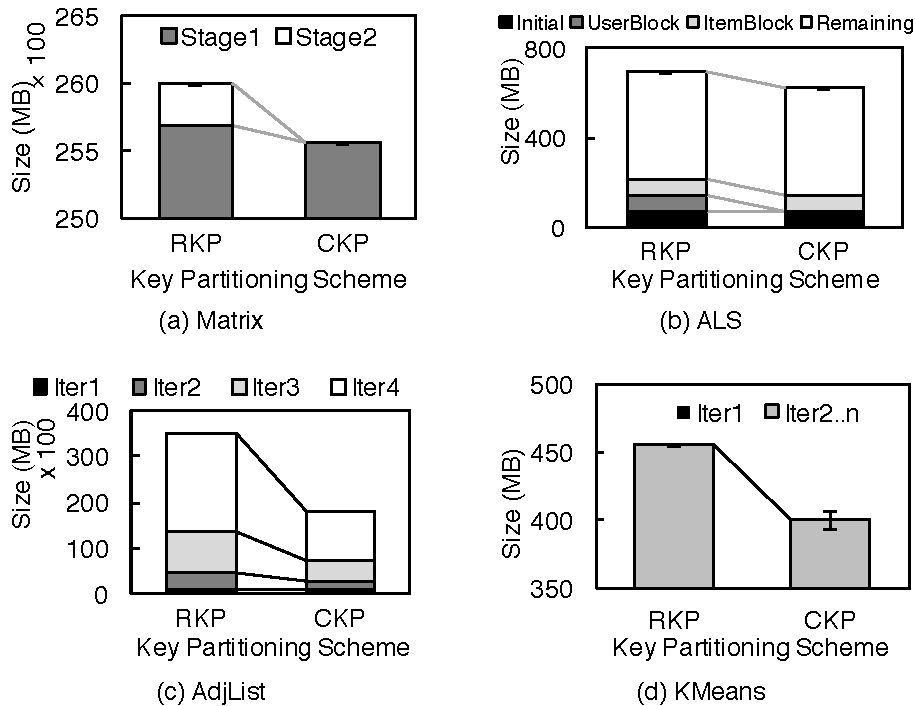
\includegraphics[width=1\columnwidth]{figure5}
\caption{Shuffle Sizes of Multiple Iterations (or Stages) in MatrixMultiplication (Matrix), MovieLensALS (ALS), MultiAdjacentList (AdjList) and KMeans Benchmarks
}
\label{fig:size}
%\vspace{-0.2in}
\end{figure}


\subsection{Shuffle Sizes Improvement} 
The results of the shuffle size of each iteration (or stage) after applying CKP and RKP in all the benchmarks are shown in Fig.~\ref{fig:size}, respectively. 

In MatrixMultiplication, CKP totally removes the shuffle operation of Stage 2 whose shuffle size is 0, and the shuffle size of Stage 1 remains closed to that of RKP (Fig.~\ref{fig:size}(a)). 
Note that when RKP is applied, the shuffle size of Stage 2 is very small as compared to Stage 1 due to the map-side combine mechanism mentioned above.
% Still, we will show that CKP has the advantage in minimizing the job completion time by eliminating the shuffle runtime overheads in the latter sub-sections. 


The benefit of applying CKP on the smaller iterative distributed operation divided based on operations can be read in Fig.~\ref{fig:size}(b).
In MovieLensALS, after applying CKP, the shuffle size for generating the user block is 0, while that for generating the item block remains almost the same as that of RKP. 
As a result, the CKP shuffle size for generating these two block is half of that of RKP. 
Because the other iterations of the distributed operations cannot be improved by CKP, 
the overall shuffle traffic CKP can decrease for the application is about 11\%.

After applying CKP in MultiAdjacentList benchmark, the shuffle size of each iteration is decreased by half beginning from Iteration 2 (Fig.~\ref{fig:size}(c)). 
The reason is that by using CKP on divided sub-operations that handle the datasets corresponding to the key $(list, tails)$, only the datasets of Key  $(heads, L_i)$ need to be shuffled.

In the KMeans benchmark, by partitioning the points into the clusters they belong to at the first few iterations, CKP decreases the overall cluster shuffle size by 12\%. 
This decrease in shuffle size is contributed by avoiding the repartition of the points that are stable to their clusters,
although not all points are fixed to their clusters in every iteration. 

Note that the shuffle sizes of the other iterations that do not apply CKP remains almost unchanged, which means that CKP can decrease the shuffle size of distributed iterations that have the confluence key dependency without introducing extra workloads to the other iterations. 
How CKP can decrease the overall shuffle traffic depends on how large the portion of data corresponding to the pure confluence subgraph take in the overall processing of the application. 
For MultiAdjacentList, the CKP can be applied to half of the operations, either appending to the head or to the tail.
While for MovieLensALS, CKP can only be applied to the operation that arrange the user-item blocks, which is only a small portion of the overall application. 
Still, it indicates the potential of applying CKP in the complicated iterative distributed applications. 


\begin{figure}[!t]
\centering
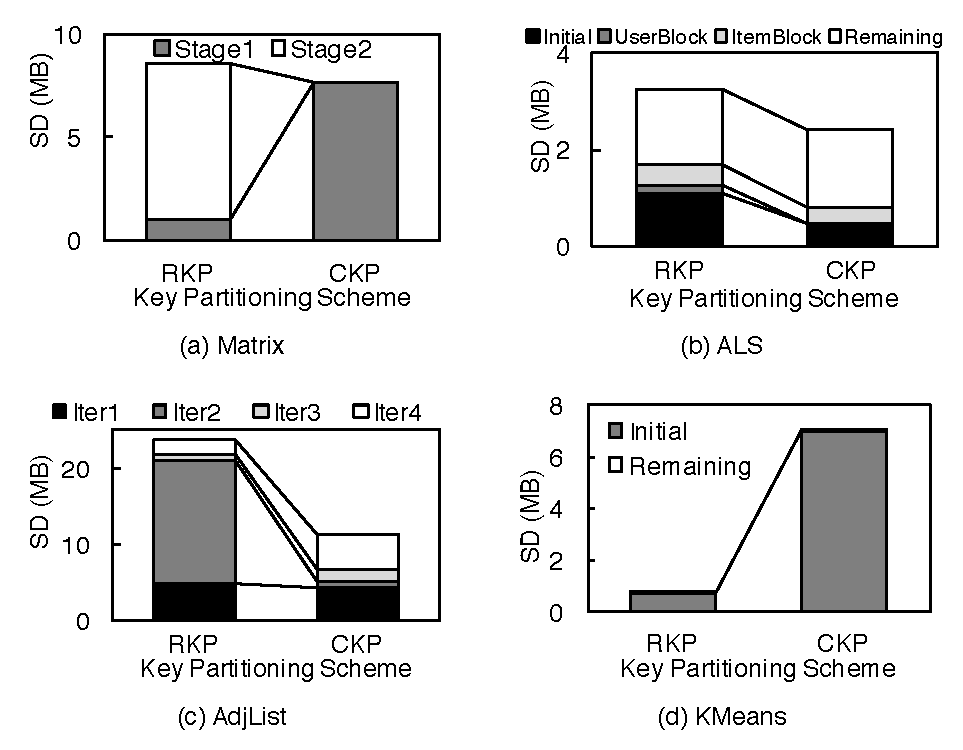
\includegraphics[width=1\columnwidth]{figure6}
\caption{Standard Deviations (SD) of the Shuffle Sizes of the Executors of Multiple Iterations (or Stages) in MatrixMultiplication (Matrix), MovieLensALS (ALS), MultiAdjacentList (AdjList) and KMeans Benchmarks
}
\label{fig:SD}
%\vspace{-0.2in}
\end{figure}


\begin{figure}[!t]
\centering
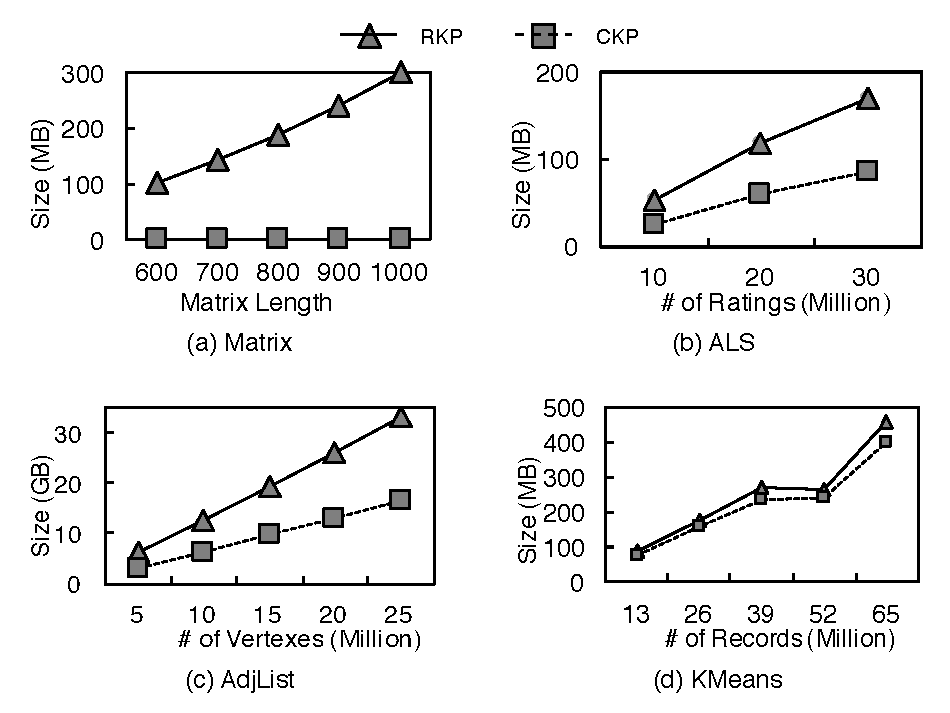
\includegraphics[width=1\columnwidth]{figure7}
\caption{Overall Shuffle Size of the Pure-Confluence-Subgraphs-Related Iterations in MatrixMultiplication (Matrix), MovieLensALS (ALS), MultiAdjacentList (AdjList) and KMeans Benchmarks with Different Input Size}
\label{fig:sizeLine}
%\vspace{-0.2in}
\end{figure}

\subsection{Workload Skew}
The standard deviations of the shuffle workloads of the executors of different benchmarks are shown in Fig.~\ref{fig:SD}. 
As expected, the workload standard deviations of the CKP-affected stages of MatrixMultiplication (Fig.~\ref{fig:SD}(a)), MovieLensALS (Fig.~\ref{fig:SD}(b)) and MultiAdjacentList (Fig.~\ref{fig:SD}(c)) are all 0. 
In the KMeans benchmark, the standard deviation of CKP is larger than that of RKP (Fig.~\ref{fig:SD}(d)). 
The reason is that the number of points belonging to each cluster varies but the number of cluster centers (32) is not large enough as compared to 
the computer nodes (16) to even the workloads of the nodes. 
If the number of cluster centers is large enough, the actual number of points partitioned to each node will get closer to the expected value, 
which is the same in every node.
Still, the standard deviation of CKP (7 MB) is small as compared to the mean shuffle size of the executors (25 MB).

For the stages that are either before or after the CKP-affected stages, the standard deviations remain almost the same as RKP, or the change is so tiny as compared to the overall shuffle size of the stage that can be ignored. 




\subsection{Scalability}
The overall shuffle sizes of the pure-confluence-subgraph-related iterations with different input sizes in various benchmarks are shown in Fig.~\ref{fig:sizeLine}. 
In MatrixMultiplication, 
the overall shuffle size of RKP increases linearly as the matrix length grows, while that of CKP is always 0. 
CKP can totally remove the shuffle workload for Stage 2 of MatrixMultiplication. 
In the other benchmarks, the shuffle sizes of CKP always keep in a fixed (or stable) ratio to those of RKP, e.g., 50\% in both MovieLensALS and MultiAdjacentList and around 88\% in KMeans. 
The result shows that CKP scales well with different volumes of input data. 
The CKP decreases the shuffle workload greatly (about 50\%) in one iteration out of the many distributed operations in the MovieLensALS application, and a little (about 12\%) but in every iteration of the distributed operations of the KMeans application. 



\section{Related Work}\label{section:relatedWork}
\textbf{Iterative distributed computing}: 
Some works \cite{gunarathne2013scalable, bu2010haloop, ekanayake2010twister} improved the distributed frameworks for the iterative MapReduce-like computing by extended the programming interfaces to support multiple map and reduce phases. 
The general idea was to cache the output data of each iteration for the next iteration. 
Spark \cite{zaharia2012resilient} provided more kinds of operation interfaces and supported a series of transformations on the distributed input datasets in the memory by the concept of resilient distributed dataset. 
These iterative distributed frameworks tried to minimize the I/O overhead by storing the intermediate data of each iteration in the memory, instead of in the disk like Hadoop. 
However, they did not consider the heavy network workload during the shuffle operations. 
Inheriting the benefit of fast memory I/O speed, Confluence decreases the shuffle sizes and alleviate the network workload by considering the key dependency of multiple relational iterations. 

\textbf{Parallel\&Distributed algorithms optimization}: Lots of work has been conducted on the optimization of parallel\&distributed machine learning algorithms~\cite{bekkerman2011scaling} and science computing \cite{kiran2013verification, mensink2012metric}, including the matrix multiplication methods~\cite{buluc2012parallel, ballard2012communication}. 
Generally, they focused on optimizing the algorithm itself by decomposing the tasks to increase the task parallelism and removing the synchronization boundary between the I/O-intensive tasks and compute-intensive tasks. 
Sarma et al. \cite{Sarma:2013:ULB} represented the map-and-reduce communication cost as the number of data entries needed to generate from the map input for the distributed application with a given parallelism factor. 
To decrease the communication cost for a specific distributed application, one need redesign the distributed program itself, operating with the proper parallelism factor. 
The term of communication cost is slightly different from the shuffle size in this paper, where the communication cost is the transfer size of data between different reduce workers, while the shuffle size transfer size of data between different computer nodes. 
The algorithms with the minimum communication cost can further decrease the shuffle size by considering the key dependency of the datasets in multiple iterations. 
ShuffleWatcher~\cite{faraz2014shufflewatcher} scheduled the locality of the map tasks and the reduce tasks to decrease shuffle inter-node traffic for the single 
iteration of the MapReduce jobs, but it did not provide the solution for iterative distributed operations. 


\textbf{Datacenter networking for shuffle}: 
In datacenters, various networking scheduling algorithms were proposed to improve the shuffle throughput for different performance goals \cite{greenberg2009vl2,popa2012faircloud,shieh2011sharing,chowdhury2011managing}.  
Confluence does not concern with the underlying network level. However, by decreasing the shuffle workload, the shuffle tasks applying the confluence key partitioning scheme can work on these shuffle-optimized datacenter networks seamlessly and gain more performance increase.    

\textbf{Skew\&Straggler}: 
The distributed computing paradigms like MapReduce adopted the data locality principle, either to place the computing tasks closed to data locations in priority to reduce the traffic workloads of data migration \cite{dean2008mapreduce, zaharia2008improving} or to avoid the unbalanced allocation of workloads by considering the compute skew problems \cite{kwon2010skew, kwon2012skewtune}. 
They concerned with the placing of map tasks where the required input data are self-contained.
As the input data of each shuffle task are distributed across the cluster, such task-to-data approach cannot help in the shuffle tasks. 
Confluence localizes the data and tasks by partitioning the data corresponding to each pure confluence subgraph with multiple shuffle iterations in the same node, which eliminates the shuffle traffic of the following iterations while not impacting the balance of workloads.
Aaron et al. \cite{Harlap:2016:ASP} addressed the problem of stragglers in iterative machine learning. If the unbalance in the granule of pure confluence subgraph does exist for some particular dataset or algorithm, the partitioning scheme of the pure confluence subgraph can be manually specified by the user to prevent stragglers. 

\textbf{DAG scheduling}: 
Similar to the DAG task scheduling algorithms \cite{sakellariou2004hybrid, zhao2006scheduling, spark-dagscheduler, isard2007dryad} that schedule the tasks to based on the task dependency graph, Confluence optimizes the partition location based on the key dependency graph. 
The difference is, in terms of the goal, that the DAG task scheduling algorithms tried to parallel the execution of jobs that are not depended on each other to increase parallelism, while Confluence isolates the partitions of the data with dependency relationship in multiple shuffle iterations to reduce the network traffic. 


\section{Conclusion and Future Work}\label{section:conclusion}
We have presented Confluence Key Partitioning scheme, the first work on decreasing the shuffle size of
iterative distributed operations leveraging the key dependency. 
Confluence guides the data partitioning across different iterations based on the key dependency graph, 
which is constructed based on the iterative key dependency.
%We use Confluence to partition the datasets to avoid undesired network traffic across multiple iterations during the shuffle operations. 
Confluence greatly decreases the overall shuffle size while not introducing the workload skew side effect for a variety of distributed operations
in the fields of scientific computing, machine learning, data
analysis, etc.



% An example of a floating figure using the graphicx package.
% Note that \label must occur AFTER (or within) \caption.
% For figures, \caption should occur after the \includegraphics.
% Note that IEEEtran v1.7 and later has special internal code that
% is designed to preserve the operation of \label within \caption
% even when the captionsoff option is in effect. However, because
% of issues like this, it may be the safest practice to put all your
% \label just after \caption rather than within \caption{}.
%
% Reminder: the "draftcls" or "draftclsnofoot", not "draft", class
% option should be used if it is desired that the figures are to be
% displayed while in draft mode.
%
%\begin{figure}[!t]
%\centering
%\includegraphics[width=2.5in]{myfigure}
% where an .eps filename suffix will be assumed under latex, 
% and a .pdf suffix will be assumed for pdflatex; or what has been declared
% via \DeclareGraphicsExtensions.
%\caption{Simulation results for the network.}
%\label{fig_sim}
%\end{figure}

% Note that IEEE typically puts floats only at the top, even when this
% results in a large percentage of a column being occupied by floats.
% However, the Computer Society has been known to put floats at the bottom.


% An example of a double column floating figure using two subfigures.
% (The subfig.sty package must be loaded for this to work.)
% The subfigure \label commands are set within each subfloat command,
% and the \label for the overall figure must come after \caption.
% \hfil is used as a separator to get equal spacing.
% Watch out that the combined width of all the subfigures on a 
% line do not exceed the text width or a line break will occur.
%
%\begin{figure*}[!t]
%\centering
%\subfloat[Case I]{\includegraphics[width=2.5in]{box}%
%\label{fig_first_case}}
%\hfil
%\subfloat[Case II]{\includegraphics[width=2.5in]{box}%
%\label{fig_second_case}}
%\caption{Simulation results for the network.}
%\label{fig_sim}
%\end{figure*}
%
% Note that often IEEE papers with subfigures do not employ subfigure
% captions (using the optional argument to \subfloat[]), but instead will
% reference/describe all of them (a), (b), etc., within the main caption.
% Be aware that for subfig.sty to generate the (a), (b), etc., subfigure
% labels, the optional argument to \subfloat must be present. If a
% subcaption is not desired, just leave its contents blank,
% e.g., \subfloat[].


% An example of a floating table. Note that, for IEEE style tables, the
% \caption command should come BEFORE the table and, given that table
% captions serve much like titles, are usually capitalized except for words
% such as a, an, and, as, at, but, by, for, in, nor, of, on, or, the, to
% and up, which are usually not capitalized unless they are the first or
% last word of the caption. Table text will default to \footnotesize as
% IEEE normally uses this smaller font for tables.
% The \label must come after \caption as always.
%
%\begin{table}[!t]
%% increase table row spacing, adjust to taste
%\renewcommand{\arraystretch}{1.3}
% if using array.sty, it might be a good idea to tweak the value of
% \extrarowheight as needed to properly center the text within the cells
%\caption{An Example of a Table}
%\label{table_example}
%\centering
%% Some packages, such as MDW tools, offer better commands for making tables
%% than the plain LaTeX2e tabular which is used here.
%\begin{tabular}{|c||c|}
%\hline
%One & Two\\
%\hline
%Three & Four\\
%\hline
%\end{tabular}
%\end{table}


% Note that the IEEE does not put floats in the very first column
% - or typically anywhere on the first page for that matter. Also,
% in-text middle ("here") positioning is typically not used, but it
% is allowed and encouraged for Computer Society conferences (but
% not Computer Society journals). Most IEEE journals/conferences use
% top floats exclusively. 
% Note that, LaTeX2e, unlike IEEE journals/conferences, places
% footnotes above bottom floats. This can be corrected via the
% \fnbelowfloat command of the stfloats package.



% if have a single appendix:
%\appendix[Proof of the Zonklar Equations]
% or
%\appendix  % for no appendix heading
% do not use \section anymore after \appendix, only \section*
% is possibly needed

% use appendices with more than one appendix
% then use \section to start each appendix
% you must declare a \section before using any
% \subsection or using \label (\appendices by itself
% starts a section numbered zero.)
%


%\appendices
%\section{Proof of the First Zonklar Equation}
%Appendix one text goes here.
%
%% you can choose not to have a title for an appendix
%% if you want by leaving the argument blank
%\section{}
%Appendix two text goes here.
%
%
%% use section* for acknowledgment
%\ifCLASSOPTIONcompsoc
%  % The Computer Society usually uses the plural form
%  \section*{Acknowledgments}
%\else
%  % regular IEEE prefers the singular form
%  \section*{Acknowledgment}
%\fi
%
%
%The authors would like to thank...


% Can use something like this to put references on a page
% by themselves when using endfloat and the captionsoff option.
%\ifCLASSOPTIONcaptionsoff
%  \newpage
%\fi



% trigger a \newpage just before the given reference
% number - used to balance the columns on the last page
% adjust value as needed - may need to be readjusted if
% the document is modified later
%\IEEEtriggeratref{22}
% The "triggered" command can be changed if desired:
%\IEEEtriggercmd{\enlargethispage{-5in}}

% references section

% can use a bibliography generated by BibTeX as a .bbl file
% BibTeX documentation can be easily obtained at:
% http://www.ctan.org/tex-archive/biblio/bibtex/contrib/doc/
% The IEEEtran BibTeX style support page is at:
% http://www.michaelshell.org/tex/ieeetran/bibtex/
% \bibliographystyle{IEEEtran}
% % argument is your BibTeX string definitions and bibliography database(s)
% \bibliography{IEEELonger}
%
% <OR> manually copy in the resultant .bbl file
% set second argument of \begin to the number of references
% (used to reserve space for the reference number labels box)
%\begin{thebibliography}{1}
% Generated by IEEEtran.bst, version: 1.13 (2008/09/30)
\begin{thebibliography}{10}
\providecommand{\url}[1]{#1}
\csname url@samestyle\endcsname
\providecommand{\newblock}{\relax}
\providecommand{\bibinfo}[2]{#2}
\providecommand{\BIBentrySTDinterwordspacing}{\spaceskip=0pt\relax}
\providecommand{\BIBentryALTinterwordstretchfactor}{4}
\providecommand{\BIBentryALTinterwordspacing}{\spaceskip=\fontdimen2\font plus
\BIBentryALTinterwordstretchfactor\fontdimen3\font minus
  \fontdimen4\font\relax}
\providecommand{\BIBforeignlanguage}[2]{{%
\expandafter\ifx\csname l@#1\endcsname\relax
\typeout{** WARNING: IEEEtran.bst: No hyphenation pattern has been}%
\typeout{** loaded for the language `#1'. Using the pattern for}%
\typeout{** the default language instead.}%
\else
\language=\csname l@#1\endcsname
\fi
#2}}
\providecommand{\BIBdecl}{\relax}
\BIBdecl

\bibitem{Malewicz:2010:PSL}
G.~Malewicz et al., ``Pregel: A system for large-scale graph processing,'' in
  \emph{Proceedings of the ACM SIGMOD International Conference on Management of
  Data}, New York, NY, USA, 2010, pp. 135--146.

\bibitem{Lu:2014:LDG}
Y.~Lu et al., ``Large-scale distributed graph computing
  systems: An experimental evaluation,'' \emph{Proceedings of the VLDB
  Endowment}, vol.~8, no.~3, pp. 281--292, Nov. 2014.

\bibitem{thusoo2009hive}
A.~Thusoo et al., ``Hive: A warehousing solution over a map-reduce
  framework,'' \emph{Proceeding of VLDB Endowment}, vol.~2, no.~2, pp.
  1626--1629, 2009.

\bibitem{Yu:2008:DSG}
Y.~Yu et al., ``Dryadlinq: A system for general-purpose distributed
  data-parallel computing using a high-level language,'' in \emph{Proceedings
  of the 8th USENIX Symposium on Operating Systems Design and Implementation},
  2008, pp. 1--14.

\bibitem{Armbrust:2015:SSR}
M.~Armbrust et al., ``Spark sql: Relational
  data processing in spark,'' in \emph{Proceedings of the 2015 ACM SIGMOD
  International Conference on Management of Data}, ser. SIGMOD '15.\hskip 1em
  plus 0.5em minus 0.4em\relax New York, NY, USA: ACM, 2015, pp. 1383--1394.

\bibitem{low2012distributed}
Y.~Low et al.,
  ``Distributed graphlab: A framework for machine learning and data mining in
  the cloud,'' \emph{Proceedings of the VLDB Endowment}, vol.~5, no.~8, pp.
  716--727, 2012.

\bibitem{kraska2013mlbase}
T.~Kraska et al., ``Mlbase: A distributed machine-learning system,'' in
  \emph{Conference on Innovative Data Systems Research (CIDR)}, vol.~1, 2013,
  pp. 2--1.

\bibitem{vavilapalli2013apache}
V.~K. Vavilapalli et al., ``Apache hadoop yarn: Yet another
  resource negotiator,'' in \emph{Proceedings of the 4th ACM Annual Symposium
  on Cloud Computing}, New York, NY, USA, 2013, pp. 5:1--5:16.

\bibitem{hindman2011mesos}
B.~Hindman et al., ``Mesos: A platform for fine-grained resource
  sharing in the data center.'' in \emph{Proceedings of the 8th USENIX
  Symposium on Networked Systems Design and Implementation}, vol.~11, 2011, pp.
  22--22.

\bibitem{isard2007dryad}
M.~Isard et al., ``Dryad: Distributed
  data-parallel programs from sequential building blocks,'' in
  \emph{Proceedings of the 2nd ACM SIGOPS/EuroSys European Conference on
  Computer Systems}, New York, NY, USA, 2007, pp. 59--72.

\bibitem{dean2008mapreduce}
J.~Dean and S.~Ghemawat, ``Mapreduce: Simplified data processing on large
  clusters,'' \emph{Communications of the ACM}, vol.~51, no.~1, pp. 107--113,
  2008.

\bibitem{shvachko2010hadoop}
K.~Shvachko et al., ``The hadoop distributed file
  system,'' in \emph{Proceedings of the IEEE 26th Symposium on Mass Storage
  Systems and Technologies}.\hskip 1em plus 0.5em minus 0.4em\relax IEEE, 2010,
  pp. 1--10.

\bibitem{chen2011case}
Y.~Chen et al., ``The case for evaluating
  mapreduce performance using workload suites,'' in \emph{IEEE 19th
  International Symposium on Modeling, Analysis \& Simulation of Computer and
  Telecommunication Systems}, 2011, pp. 390--399.

\bibitem{chowdhury2011managing}
M.~Chowdhury et al., ``Managing data
  transfers in computer clusters with orchestra,'' in \emph{Proceedings of the
  ACM SIGCOMM Conference}.\hskip 1em plus 0.5em minus 0.4em\relax New York, NY,
  USA: ACM, 2011, pp. 98--109.

\bibitem{al2010hedera}
M.~Al-Fares et al., ``Hedera:
  Dynamic flow scheduling for data center networks.'' in \emph{Proceedings of
  the 7th USENIX conference on Networked Systems Design and Implementation},
  vol.~10, 2010, pp. 19--19.

\bibitem{bu2010haloop}
Y.~Bu et al., ``Haloop: efficient iterative
  data processing on large clusters,'' \emph{Proceedings of the VLDB
  Endowment}, vol.~3, no. 1-2, pp. 285--296, 2010.

\bibitem{zaharia2012resilient}
M.~Zaharia et al., ``Resilient distributed datasets: A fault-tolerant
  abstraction for in-memory cluster computing,'' in \emph{Proceedings of the
  9th USENIX conference on Networked Systems Design and Implementation}, 2012,
  pp. 2--2.

\bibitem{ekanayake2010twister}
J.~Ekanayake et al.,
  ``Twister: a runtime for iterative mapreduce,'' in \emph{Proceedings of the
  19th ACM International Symposium on High Performance Distributed Computing},
  2010, pp. 810--818.

\bibitem{sakellariou2004hybrid}
R.~Sakellariou and H.~Zhao, ``A hybrid heuristic for dag scheduling on
  heterogeneous systems,'' in \emph{Proceedings of 18th IEEE International
  Parallel and Distributed Processing Symposium}, 2004, pp. 111--.

\bibitem{zhao2006scheduling}
H.~Zhao and R.~Sakellariou, ``Scheduling multiple dags onto heterogeneous
  systems,'' in \emph{Proceedings of 20th IEEE International Parallel and
  Distributed Processing Symposium}, 2006, pp. 14--.

\bibitem{movielensals}
\BIBentryALTinterwordspacing
``Movielensals spark submit 2014.'' [Online]. Available:
  \url{https://databricks-training.s3.amazonaws.com/movie-recommendation-with-mllib.html}
\BIBentrySTDinterwordspacing

\bibitem{multiAdjList}
\BIBentryALTinterwordspacing
``Multiadjacentlist benchmark.'' [Online]. Available:
  \url{https://github.com/liangfengsid/MultiAdjacentList}
\BIBentrySTDinterwordspacing

\bibitem{kmeans}
\BIBentryALTinterwordspacing
``Spark kmeans benchmark.'' [Online]. Available:
  \url{http://spark.apache.org/docs/latest/mllib-clustering.html}
\BIBentrySTDinterwordspacing

\bibitem{gideon}
\BIBentryALTinterwordspacing
``Hku gideon-ii cluster.'' [Online]. Available:
  \url{http://i.cs.hku.hk/\%7Eclwang/Gideon-II/}
\BIBentrySTDinterwordspacing

\bibitem{gunarathne2013scalable}
T.~Gunarathne et al., ``Scalable parallel computing on
  clouds using twister4azure iterative mapreduce,'' \emph{Future Generation
  Computer Systems}, vol.~29, no.~4, pp. 1035--1048, 2013.

\bibitem{bekkerman2011scaling}
R.~Bekkerman, M.~Bilenko, and J.~Langford, \emph{Scaling up machine learning:
  Parallel and distributed approaches}.\hskip 1em plus 0.5em minus 0.4em\relax
  Cambridge University Press, 2011.

\bibitem{kiran2013verification}
M.~Kiran, A.~Kumar, and B.~Prathap, ``Verification and validation of parallel
  support vector machine algorithm based on mapreduce program model on hadoop
  cluster,'' in \emph{IEEE International Conference on Advanced Computing and
  Communication Systems}, 2013, pp. 1--6.

\bibitem{mensink2012metric}
T.~Mensink et al., ``Metric learning for
  large scale image classification: Generalizing to new classes at near-zero
  cost,'' in \emph{Computer Vision--ECCV 2012}.\hskip 1em plus 0.5em minus
  0.4em\relax Springer, 2012, pp. 488--501.

\bibitem{buluc2012parallel}
A.~Buluc and J.~R. Gilbert, ``Parallel sparse matrix-matrix multiplication and
  indexing: Implementation and experiments,'' \emph{SIAM Journal on Scientific
  Computing}, vol.~34, no.~4, pp. C170--C191, 2012.

\bibitem{ballard2012communication}
G.~Ballard et al.,
  ``Communication-optimal parallel algorithm for strassen's matrix
  multiplication,'' in \emph{Proceedings of the 24th annual ACM Symposium on
  Parallelism in Algorithms and Architectures}, 2012, pp. 193--204.

\bibitem{Sarma:2013:ULB}
A.~D. Sarma et al., ``Upper and lower
  bounds on the cost of a map-reduce computation,'' \emph{Proceedings of the
  VLDB Endowment}, vol.~6, no.~4, pp. 277--288, 2013.

\bibitem{faraz2014shufflewatcher}
F.~Ahmad et al.,
  ``Shufflewatcher: Shuffle-aware scheduling in multi-tenant mapreduce
  clusters,'' in \emph{2014 USENIX Annual Technical Conference (USENIX ATC
  14)}.\hskip 1em plus 0.5em minus 0.4em\relax Philadelphia, PA: USENIX
  Association, Jun. 2014, pp. 1--13.

\bibitem{greenberg2009vl2}
A.~Greenberg et al., ``Vl2: a scalable and flexible data center
  network,'' in \emph{Communication of the ACM}, vol.~54, no.~3, 2011, pp.
  95--104.

\bibitem{popa2012faircloud}
L.~Popa et al.,
  ``Faircloud: sharing the network in cloud computing,'' in \emph{Proceedings
  of the ACM SIGCOMM conference on Applications, technologies, architectures,
  and protocols for computer communication}, 2012, pp. 187--198.

\bibitem{shieh2011sharing}
A.~Shieh et al., ``Sharing the data
  center network,'' in \emph{Proceedings of the 8th USENIX Symposium on
  Networked Systems Design and Implementation}, 2011, pp. 309--322.

\bibitem{zaharia2008improving}
M.~Zaharia et al., ``Improving
  mapreduce performance in heterogeneous environments,'' in \emph{Proceedings
  of the 8th USENIX Symposium on Operating Systems Design and Implementation},
  2008, pp. 29--42.

\bibitem{kwon2010skew}
Y.~Kwon et al., ``Skew-resistant parallel
  processing of feature-extracting scientific user-defined functions,'' in
  \emph{Proceedings of the 1st ACM Symposium on Cloud Computing}.\hskip 1em
  plus 0.5em minus 0.4em\relax ACM, 2010, pp. 75--86.

\bibitem{kwon2012skewtune}
Y.~Kwon et al., ``Skewtune: mitigating skew in mapreduce applications,'' in
  \emph{Proceedings of the ACM SIGMOD International Conference on Management of
  Data}, 2012, pp. 25--36.

\bibitem{Harlap:2016:ASP}
A.~Harlap et al., ``Addressing the straggler problem for iterative convergent
  parallel ml,'' in \emph{Proceedings of the Seventh ACM Symposium on Cloud
  Computing}, ser. SoCC '16.\hskip 1em plus 0.5em minus 0.4em\relax New York,
  NY, USA: ACM, 2016, pp. 98--111.

\bibitem{spark-dagscheduler}
\BIBentryALTinterwordspacing
Spark job scheduling: Dagscheduler. [Online]. Available:
  \url{https://spark.apache.org/docs/1.4.0/job-scheduling.html}
\BIBentrySTDinterwordspacing

\end{thebibliography}

%
%\bibitem{IEEEhowto:kopka}
%H.~Kopka and P.~W. Daly, \emph{A Guide to \LaTeX}, 3rd~ed.\hskip 1em plus
%  0.5em minus 0.4em\relax Harlow, England: Addison-Wesley, 1999.
%
%\end{thebibliography}

% biography section
% 
% If you have an EPS/PDF photo (graphicx package needed) extra braces are
% needed around the contents of the optional argument to biography to prevent
% the LaTeX parser from getting confused when it sees the complicated
% \includegraphics command within an optional argument. (You could create
% your own custom macro containing the \includegraphics command to make things
% simpler here.)
%\begin{IEEEbiography}[{\includegraphics[width=1in,height=1.25in,clip,keepaspectratio]{mshell}}]{Michael Shell}
% or if you just want to reserve a space for a photo:


\begin{IEEEbiography}[{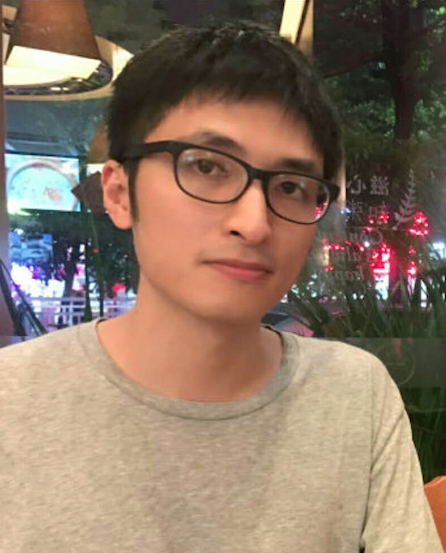
\includegraphics[width=1in,height=1.25in,clip,keepaspectratio]{author1}}]{Feng Liang}
is currently a PhD candidate in Department of Computer Science, The University of Hong Kong. He received his bachelor's degree in software engineering in Nanjing University in 2012. His research interests are mainly on distributed file systems, distributed computing, and machine learning. He is recently undertaking the research project on distributed deep learning.
[homepage] i.cs.hku.hk/\%7Efliang
\end{IEEEbiography}

\begin{IEEEbiography}[{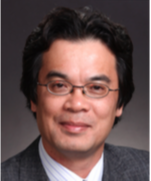
\includegraphics[width=1in,height=1.25in,clip,keepaspectratio]{author2}}]{Francis C.M. Lau}
received his PhD in computer science from the University of Waterloo in 1986. He has been a faculty member of the Department of Computer Science, The University of Hong Kong since 1987, where he served as the department chair from 2000 to 2005. He is now Associate Dean of Faculty of Engineering, the University of Hong Kong. He was a honorary chair professor in the Institute of Theoretical Computer Science of Tsinghua University from 2007 to 2010. His research interests include
computer systems and networking, algorithms, HCI, and application of IT to arts. He is the editor-in-chief of the Journal of Interconnection Networks.
[homepage] i.cs.hku.hk/\%7Efcmlau
\end{IEEEbiography}

\begin{IEEEbiography}[{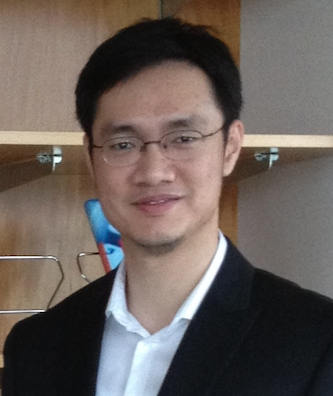
\includegraphics[width=1in,height=1.25in,clip,keepaspectratio]{author3}}]{Heming Cui}
is an assistant professor in Computer Science of HKU. His research interests are in operating systems, programming languages, distributed systems, and cloud computing, with a particular focus on building software infrastructures and tools to improve reliability and security of real-world software. 
[homepage] i.cs.hku.hk/\%7Eheming
\end{IEEEbiography}

\begin{IEEEbiography}[{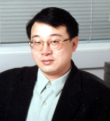
\includegraphics[width=1in,height=1.25in,clip,keepaspectratio]{author4}}]{Cho-Li Wang}
is currently a Professor in the Department of Computer Science at The
University of Hong Kong. He graduated with a B.S. degree in Computer Science and
Information Engineering from National Taiwan University in 1985 and a Ph.D.
degree in Computer Engineering from University of Southern California in 1995. Prof.
Wang’s research is broadly in the areas of parallel architecture, software systems for
Cluster computing, and virtualization techniques for Cloud computing. His recent
research projects involve the development of parallel software systems for
multicore/GPU computing and multi-kernel operating systems for future manycore
processor. Prof. Wang has published more than 150 papers in various peer reviewed
journals and conference proceedings. He is/was on the editorial boards of several scholarly
journals, including IEEE Transactions on Cloud Computing (2013-), IEEE
Transactions on Computers (2006-2010).
[homepage] i.cs.hku.hk/\%7Eclwang
\end{IEEEbiography}

% insert where needed to balance the two columns on the last page with
% biographies
%\newpage



% You can push biographies down or up by placing
% a \vfill before or after them. The appropriate
% use of \vfill depends on what kind of text is
% on the last page and whether or not the columns
% are being equalized.

%\vfill

% Can be used to pull up biographies so that the bottom of the last one
% is flush with the other column.
%\enlargethispage{-5in}



% that's all folks
\end{document}


